%Requires the memoir class 
\documentclass[oneside,11pt]{memoir}

%\usepackage{mathptmx}  % Times New Roman, but if you have Garamond 
                        % then use it;
                        % you are writing a book, not a newspaper column

\DoubleSpacing        % memoir's double spacing
\usepackage{rice}     % rice thesis package 


\usepackage{graphicx}
\usepackage{rotating}
\usepackage{amsmath}
\usepackage{amssymb}
\usepackage{bm}

\usepackage{txfonts}  % I used this one to summon the symbol for \lambdabar
\usepackage{lmodern}

\usepackage[numbers,compress]{natbib}

\usepackage{hyperref}
%\hypersetup{colorlinks=false}



\usepackage{memhfixc}

%%%%%%%%%%%%%%%%%%%%%%%%%%%%%%%%%%%%%%%%%%%%%%%%%%%%%%%%%%%%%%%%%%%
%%%% Definition of command shortcuts                           %%%%
%%%%%%%%%%%%%%%%%%%%%%%%%%%%%%%%%%%%%%%%%%%%%%%%%%%%%%%%%%%%%%%%%%%

\newcommand{\twos}[1]
     {\ensuremath{\hspace{-1pt}2\hspace{0.5pt}\hspace{0pt}S_{#1}\hspace{-1pt}}}
\newcommand{\twop}[1]
     {\ensuremath{\hspace{-1pt}2\hspace{0.5pt}\hspace{0pt}P_{#1}\hspace{-1pt}}}
\newcommand{\trep}[1]
     {\ensuremath{\hspace{-1pt}3\hspace{0.5pt}\hspace{0pt}P_{#1}\hspace{-1pt}}}

\newcommand{\cm}{\ensuremath{,\hspace{1pt}}}
\newcommand{\f}[1]{\ensuremath{F\hspace{-5pt}=\hspace{-4pt}#1}}
\newcommand{\mf}[1]{\ensuremath{m_{F}\hspace{-4pt}=\hspace{-4pt}#1}}
\newcommand{\mj}[1]{\ensuremath{m_{J}\hspace{-5pt}=\hspace{-4pt}#1}}
\newcommand{\mcm}{\ensuremath{\hspace{-4pt}}}

\newcommand{\red}
     {\ensuremath{ \twos{1/2}\hspace{-0.0pt}\rightarrow\hspace{-0.0pt}\twop{3/2} }\ }
\newcommand{\uv}
     {\ensuremath{ \twos{1/2}\hspace{-0.0pt}\rightarrow\hspace{-0.0pt}\trep{3/2} }\ }

\newcommand{\TD}{\ensuremath{ T_{D} }}
\newcommand{\TR}{\ensuremath{ T_{R} }}
\newcommand{\TF}{\ensuremath{ T_{F} }}

\newcommand{\one}{\ensuremath{|1\rangle }\ }
\newcommand{\two}{\ensuremath{|2\rangle }\ }

\newcommand{\isat}{ \ensuremath{ I_{\mathrm{sat}} } } 
\newcommand{\isatred}{ \ensuremath{ I_{sat\text{(red)}} } } 
\newcommand{\isatuv}{ \ensuremath{ I_{sat\text{(uv)}} } } 
\newcommand{\li} {\ensuremath{^{6}}Li\ }
\newcommand{\kb} { \ensuremath{k_{\mathrm{B}}}}

%%%%%%%%%%%%%%%%%%%%%%%%%%%%%%%%%%%%%%%%%%%%%%%%%%%%%%%%%%%%%%%%%%%

\newcommand{\bv}[1]{\ensuremath{\bm{#1}}}
\newcommand{\vo}{\ensuremath{V_{0}}}
\newcommand{\vvo}{\ensuremath{v_{0}}}
\newcommand{\bvo}{\ensuremath{\bv{V}_{0}}}
\newcommand{\er}{\ensuremath{E_{r}}}
\newcommand{\Lc}{\ensuremath{L_{\mathrm{c}}}}
\newcommand{\dsig}[1]{\ensuremath{ \frac{ d\,\sigma_{#1} }{d\,\Omega} }}
\newcommand{\dbl}{\ensuremath{ \uparrow\! \downarrow \, }}
\newcommand{\spup}{\ensuremath{ \uparrow }}
\newcommand{\spdn}{\ensuremath{ \downarrow}}




%%%%%%%%%%%%%%%%%%%%%%%%%%%%%%%%%%%%%%%%%%%%%%%%%%%%%%%%%%%%%%%%%%%
%%%%%%%%%%%%%%%%%%%%%%%%%%%%%%%%%%%%%%%%%%%%%%%%%%%%%%%%%%%%%%%%%%%
%%%%%%%%%%%%%%%%%%%%%%%%%%%%%%%%%%%%%%%%%%%%%%%%%%%%%%%%%%%%%%%%%%%


\DoubleSpacing

\begin{document}

\maxtocdepth{subsection}   % put everything into the ToC
\pagestyle{plain}          % pagestyle for the prelims

\frontmatter
\thetitlepage

%%%%%%%%%%%%%%%%%%%%%%%%%%%%%%%%%%%%%%%%%%%%%%%%%%%%%%%%%%%%%%%%%%%

% put your abstract here

\riceabstract
\pagestyle{empty}  % Rice requires no page numbering in the abstract

Abstract goes here. 

\pagestyle{plain} % Restore page numbering.

% put your acknowledgments here 
 
\riceacknowledgments

Acknowledgments go here. 

%% \setdedication{ text } % if you want a dedication
%\ricededication

%\tableofcontents
\tableofcontents*  % The starred version does not add "Table of Contents" to the Table of Contents
                   % I prefer it this way


% I don't find these two particularly useful
%% \listoffigures  % if you want to include a list of figures  
%% \listoftables   % if you want to include a list of tables


%% if you have more prelim sections, then
%%%% \clearpage
%%%% \pagestyle{plain}
%%%% \prelimtitle   text % for sections after the ToC, etc, before main text


\mainmatter
\pagestyle{rice}


%% Change the spacing between paragraphs, I prefered this for readability 
\let\oldparskip\parskip
\setlength{\parskip}{0.8em}



%%%%%%%%%%%%%%%%%%%%%%%%%%%%%%%%%%%%%%%%%%%%%%%%%%%%%%%%%%%%%%%%%%%%%%%%%%%%%%%
%%%%%%%%%%%%%%%%%%%%%%%%%%%%%%%%%%%%%%%%%%%%%%%%%%%%%%%%%%%%%%%%%%%%%%%%%%%%%%%
%%%%  CHAPTER 1 
%%%%%%%%%%%%%%%%%%%%%%%%%%%%%%%%%%%%%%%%%%%%%%%%%%%%%%%%%%%%%%%%%%%%%%%%%%%%%%%
%%%%%%%%%%%%%%%%%%%%%%%%%%%%%%%%%%%%%%%%%%%%%%%%%%%%%%%%%%%%%%%%%%%%%%%%%%%%%%%

\chapter{Many body physics with ultracold atoms } 

\section{ Motivation:  Strongly correlated materials }

Most of uur experiences in the physical world can, in principle, be explained
by considering the description of the collections of positively charged nuclei
and negatively charged electrons that make up ordinary matter.    From high to
low energy this includes: neutral plasmas,  free atoms and molecules, atoms and
molecules that have condensed into liquid or glassy phases or crystallized to
form solids.   At lower energies more exotic phenomena take place, starting
with magnetism and going further to superfluidity, superconductivity and the
novel examples of modern condensed matter physics such as the fractional
quantum Hall effect, heavy electrons, high-temperature superconductors and
topological insulators.

In principle,  the correct description of all the above phenomena is contained
in the Schr\"{o}dinger equation for the interacting system of electrons and
nuclei,  where the interaction is given by the Coulomb potential. In practice,
we know that even though stating the equation is easy, there is not sufficient
computing power available in the world to solve it for systems of more than
just a few particles.  Xiao-Gang Wen, in the introduction to his
book~\cite{wen2004quantum}, points out that back in the 80's a computer with 32
MB of RAM could solve a system of 11 interacting electrons.  In the 2000's,
while computing power has increased more than 100 times, this allows for the
addition of only two more electrons to the system.  

Despite the above,  the use of the Schr\"{o}dinger equation and perturbation
theory for the description of  systems of electrons and nuclei has been very
successful over the past century.  The most prominent example of this success
is our understanding of semiconductors, which are at the root of the electronic
devices that permeate all aspects of our lives.  The remarkable success of
condensed matter physics can be traced back to the principle of adiabatic
continuity~\cite{altland2010condensed}. This principle  states that  the
low-energy excitations of an interacting system  are  \textbf{non-interacting
quasiparticles} which can be closely related to the actual particles that form
the interacting system.   This last sentence may sound confusing, but think
about a hole in the valence band of a semiconductor.  The hole corresponds to a
collective arrangement of all the electrons in the system, but we typically do
not think about it that way.  The hole is a low energy excitation of the
collection of electrons, and thus we think about it as a
\textbf{quasiparticle}, with properties that are remarkably similar to those of
a free electron albeit with a positive rather than a negative charge.  The fact
that an electron and a hole behave so similarly is not at all intuitive,
especially if one stops to think about any effects due to the  Coulomb
interaction between electrons. However, adiabatic continuity guarantees that
for practical purposes we can think of the hole simply as a positively charged
electron.  

The practical consequence of adiabatic continuity is that interactions
seemingly do not play an important role in the low-energy description of the
system.  For this reason, the free electron model of Drude and
Sommerfeld~\cite{ashcroft1976solid} is relatively successful in explaining
electrical and thermal conductivity in metals,  and also in explaining the Hall
effect.   In 1957, Landau formulated the theory of the
Fermi-Liquid~\cite{landau1965collected} and gave a solid basis to the notion of
adiabatically connected quasiparticles.  To this day, the Fermi-Liquid theory
is the default starting point for the study of Fermi systems such as
conventional metals, helium-3, and ultracold atomic Fermi gases.   

But, just as Fermi-Liquid theory is celebrated for its success, it is also
known for the phenomena that it fails to explain.   Starting in the mid 70's
and going through the 80's, the discoveries of heavy electron
superconductivity~\cite{PhysRevLett.35.1779,PhysRevLett.43.1892},  the
fractional quantum Hall effect~\cite{PhysRevLett.48.1559,PhysRevLett.50.1395},
and high-temperature superconductors~\cite{Zeitschrift.64.189} sparked a
revolution in condensed matter physics~\cite{coleman2004revolution}.   These
materials, in which the electron behavior cannot be described effectively in
terms of non-interacting electron-like quasiparticles came to be known as
\textbf{strongly correlated materials}.   Strongly correlated materials, and
the concept of emergence, introduced by P.W.~Anderson in his famous essay
``More is Different''~\cite{Anderson1972}, are at the center of modern
condensed matter physics. 

The behavior of strongly correlated materials is emergent because the
low-energy excitations of the system bear no resemblance to its constituent
particles.  This disconnect should not be so surprising, after all we are
familiar with this definition of emergence whenever a system undergoes a phase
transition.  For example, when a liquid cools down to form a crystalline solid,
continuous translational symmetry is broken.    By going across the
liquid-to-solid phase transition, adiabatic continuity is violated;
nevertheless, it is easy to mathematically identify the low energy excitations
of the system and ascribe them the character of quasiparticles.  In the case of
the crystalline solid this involves finding the normal modes of a set of
coupled oscillators; the normal modes are the quasiparticles known as phonons.
Phonons are emergent because they bear no direct resemblance to the constituent
ions that form the crystal lattice. 

Strongly correlated materials are examples of emergent phenomena in which the
origin and properties of the low-energy excitations are not as straightforward
as those of phonons in a crystalline solid.  The fractional quantum Hall state,
in which the quasiparticles carry a rational fraction of the electron charge
serves to illustrate this point.  The strong interactions between the electrons
in the quantum Hall system (electrons confined in a plane in the presence of a
very high magnetic field) make the problem intractable from the perturbative
point of view and thus \textbf{the connection between the microscopic degrees
of freedom and the collective low-energy excitations is very difficult to
establish}; certainly not as easy as the connection between small displacements
of ions about their equilibrium points in a crystal lattice and the collective
phonon modes. It was Laughlin's insight that led him to postulate the correct
wavefunction  for the quantum Hall state~\cite{PhysRevLett.50.1395}, but the
microscopic origin of the state is still under debate.   

The challenge posed by strongly correlated materials has led to great
discoveries in condensed matter physics, such as the concepts of topological
order~\cite{wen1990topological} and quantum
criticality~\cite{PhysRevB.14.1165,sachdev2011quantum}, but also many questions
remain unanswered.  Furthermore, the problem of strongly correlated materials
is only scratching the surface of what is possible and what remains to be
discovered.  New materials are being synthesized constantly.  Among the
myriad of possible materials and compounds yet to be explored by
materials scientists, one can only expect that there will be new states of
matter to be found; states with technological implications that will
revolutionize life on earth.  


\section{Quantum simulations with ultracold atoms}

We have seen that, even though the Schr\"{o}dinger equation in principle
contains a full description of a solid,  its solution is practically impossible
to compute using a classical computer due to the large amount of memory
required to represent a many-body quantum state.   
%Beyond this issue of scalability there is also the issue of interpretation of
%the results:  suppose that we were able to access the exact quantum state of
%the system and its time dependence,  what would we even do with such
%information?   It would be practically impossible to come up with experiments
%that could test the full validity of the state, thus making such knowledge
%superfluous since, after all, physics is an empirical endeavor.
The approach in condensed matter theory, rather than directly aim to solve the
complete Schr\"{o}dinger equation, is to introduce simplified effective models,
which should capture the essential features of the system under study.  The
solution of the effective model leads to an understanding of the low-energy
excitations of the system and gives clues to their microscopic origin.   

The Hubbard model, formulated half a century ago~\cite{hubbard50} contains only
the essential ingredients necessary to describe the  behavior of strongly
interacting electrons moving in a periodic lattice. It describes electrons that
can hop between sites in a lattice (with probability amplitude $t$) , and which
acquire an interaction energy ($U$) when two electrons are on the same site,
see Figure~\ref{fig:chap01hubbard}.  
\begin{figure} \centering
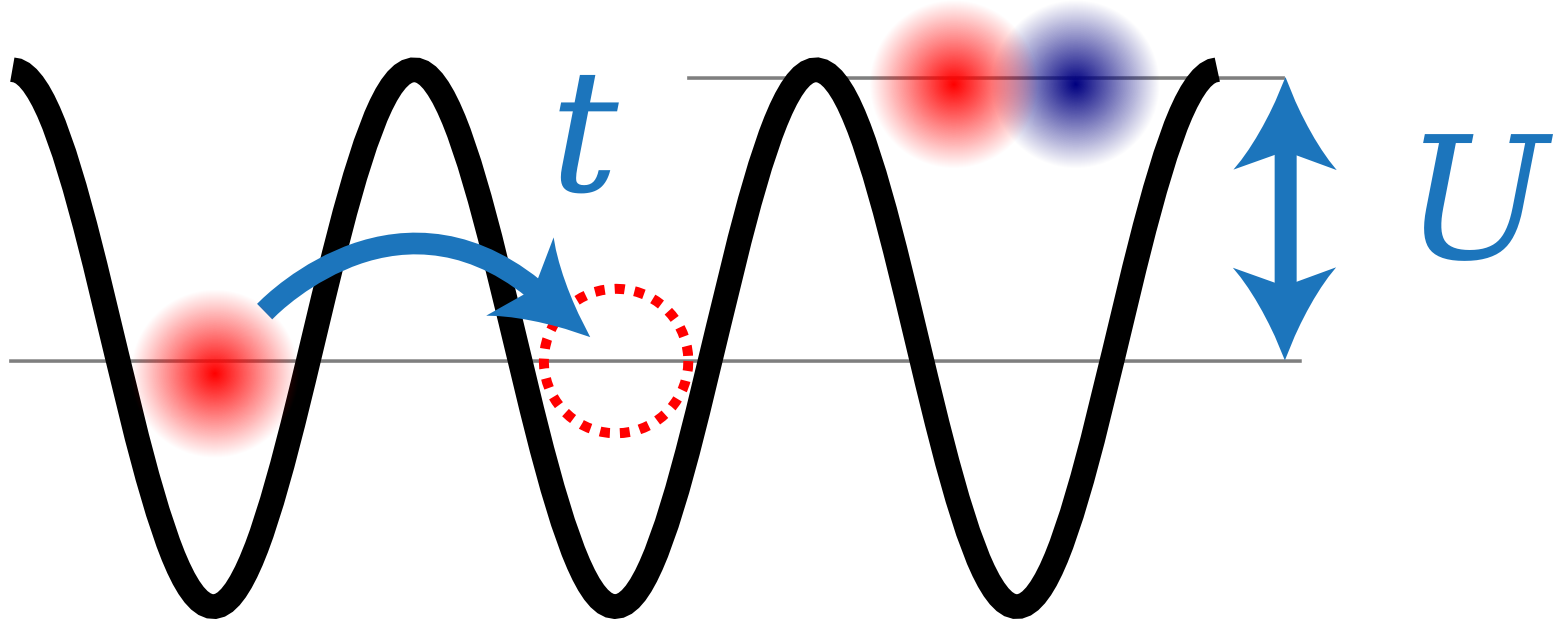
\includegraphics[width=0.4\textwidth]{../figures/hubbard/little-hubbard.png}
\caption[Hubbard model]{\small Illustration of the Hubbard model }
\label{fig:chap01hubbard}
\end{figure}
The Hubbard model is an extension of the tight-binding model, with the
interactions between electrons incorporated as the on-site energy $U$.
After its inception, it was shortly realized~\cite{Hubbard1964} that the model
could explain the Mott metal-insulator transition, which was observed in the
transition metal oxides even though conventional band theory predicted them to
be conductors.  Beyond its early success, the Hubbard model is now the
quintessential model for strongly correlated systems.  It is widely accepted as
the most viable candidate to explain high-$T_{c}$ superconductors from first
principles.   Despite this fact, its exact solution in more than one dimension
has evaded theorists for more than four decades~\cite{quintanilla2009strong}.

It is at this point that ultracold atoms enter the picture.   It turns out that
ultracold atoms in an optical lattice provide a faithful realization of the
Hubbard model~\cite{PhysRevLett.81.3108}, thus the properties exhibited by the
collection of atoms are in fact the solutions of the model.    In this way,
such systems can be used to map the phase diagram of the Hubbard model in what
is known as \textbf{quantum simulation}, an idea that was first proposed by
Richard Feynman in 1982~\cite{feynman1982simulating}. 

In a seminal paper~\cite{PhysRevLett.81.3108}, Jaksch and collaborators  showed
that Bose-Einstein condensates of atoms loaded into optical lattices could be
used as simulators of the Bose-Hubbard model.  A few years later, the superfluid
(SF) to Mott insulator (MI) phase transition, the hallmark of the Bose-Hubbard
model, was realized experimentally~\cite{Greiner2002}, and several detailed
studies of this system have followed since then~\cite{Gemelke2009,
Jimenez-Garcia2010, Trotzky2010, Mark2011, Zhang2012}.  For bosonic systems the
properties of the ground state are well understood
theoretically~\cite{freericks1994bosehubbard, trivedi1991mott,
PhysRevB.40.546};  however, experiments of atoms in lattices are starting to
shed light into the dynamics of these systems~\cite{Fukuhara2013}, which are
more difficult to address for theorists.  

Despite the remarkable advances with bosonic systems, the ultimate goal of
quantum simulation with ultracold atoms is to find the ground states of
theoretically intractable fermionic models, to see if these models can
reproduce the measured properties of strongly correlated electron systems.  In
this prescription for quantum simulation, the subject of most interest is
whether or not the Hubbard model can exhibit a $d$-wave superfluid state which
would validate it as the prime model for high-$T_{c}$
superconductors~\cite{Scalapino1995329,PhysRevLett.89.220407}.  In pursuit of
this goal, experiments have realized the Hubbard model with spin mixtures of
fermionic atoms, where two hyperfine levels of the atomic ground state play the
role of spin-up and spin-down states of the spin-$\frac{1}{2}$ electrons in
real compounds. 

In these experiments, a quantum degenerate spin-mixture of fermionic atoms is
prepared in a harmonic potential and then transferred adiabatically into an
optical lattice potential.  The lattice depth and the contact interactions
between the atoms, which together set the values for the Hubbard parameters $t$
and $U$, can be controlled almost at will by the experimenter.  The tunneling
rate $t$ is controlled  by adjusting the intensity of the lattice lasers.  The
interaction strength $U$ is controlled by setting the external magnetic field
and making use of a magnetically tunable Feshbach resonance, which offers the
possibility of realizing non-interacting samples, or samples with, arbitrarily,
large  attractive or repulsive interactions\footnote{In practice it is observed
that, for some values of the interaction strength, significant three-body
losses and the associated heating rates prevent studying the equilibrium
physics of the quantum gas~\cite{PhysRevA.85.063615}.}.  These unprecedented
control over the system parameters has allowed the realization of band
insulating states~\cite{Kohl2005} and Mott insulating
states~\cite{Jordens2008,Schneider2008} with spin-mixtures of ultracold
fermionic atoms.  However, the possibility of exploring the strongly correlated
phases of the Hubbard model has not yet been realized because the required
temperatures are out of reach for current experiments.    


 
\section{Quantum magnetism with ultracold atoms }

Even though temperatures as low as $T\simeq 0.04\,T_{F}$ can be reached with
ultracold Fermi gases in a harmonic trap, these temperatures are not low enough
to allow exploration of the strongly correlated phases of the Hubbard model.
To get an idea of the temperature scales involved, we will examine a
qualitative temperature-doping 
%($T$-$x$) 
phase diagram, which can be obtained experimentally for the cuprate
high-$T_{c}$ superconductors\footnote{See \cite{Damascelli2003} for a review of
cuprate superconductors, \cite{He2011} for a study of the onset of
superconductivity at optimal hole-doping, \cite{Jin2011} for the phase diagram
of hole-doped cuprate superconductors and \cite{Grant2011} for a more
accessible report on the subject.}, see Fig.~\ref{fig:cartoon-phasediag}.
\begin{figure} \centering
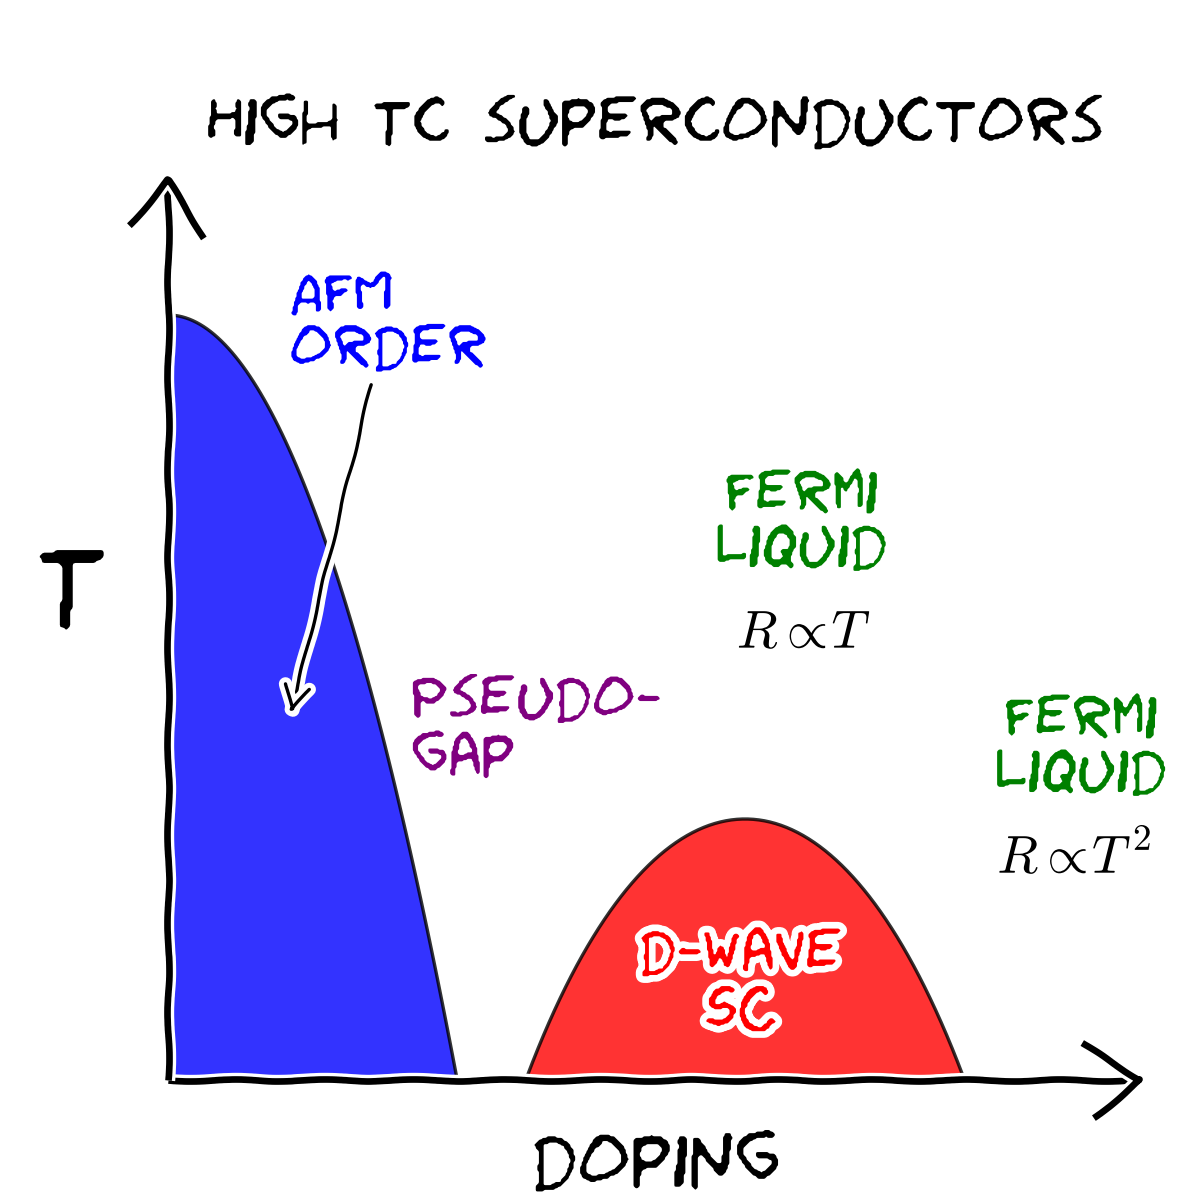
\includegraphics[width=0.4\textwidth]{../figures/hubbard/highTc.png}
\caption[Cartoon phase diagram for cuprate high-$T_{\text{C}}$
superconductors.]{\small Cartoon phase diagram for cuprate high-$T_{\text{C}}$
superconductors. The anitiferromagnetic insulator (AFM) and the Fermi liquid
with quadratic resistivity are well understood by theory, however the strange
Fermi liquid with linear resistivity and the interplay between the pseudogap
regime and the superconducting dome are issues still under
debate~\cite{Grant2011}. }
\label{fig:cartoon-phasediag}
\end{figure}

The qualitative phase diagram shows that the cuprates exhibit various
interesting phases besides the superconducting (SC) dome at intermediate
doping.   Most importantly, the undoped parent compound is an antiferromagnetic
(AFM) Mott insulator with a N\'{e}el ordering temperature that is higher than
any value of the critical temperature $T_{\text{c}}$ along the SC dome.  

The onset of AFM ordering in the cuprate parent compounds is driven by the
magnetic exchange interaction~\cite{Koch2012}, where a pair of spins can lower
their energy if they can tunnel virtually to the neighboring site.  For a
single band model, the Pauli exclusion principle dictates that this is only
possible if neighboring sites have opposing spins, as in the N\'{e}el AFM
state.  The N\'{e}el temperature $T_{N}$ is then on the order of the exchange
energy $4t^{2}/U$, which is the second-order correction (due to virtual
tunneling)  to the ground state energy of a two-site model where the
interaction $U$ is treated as a perturbation.   The undoped parent compounds,
at temperatures several times larger than $T_{N}$, will be Mott insulators with
exactly one electron per lattice site but without any kind of spin ordering.
As $T_{N}$ is approached, AFM correlations between the spins start to develop.  

To put some estimates on the values of $T_{N}$ and $T_{c}$, let's consider the
most common high-$T_{c}$ superconductor~\cite{Milton2010},
YBa$_{2}$Cu$_{3}$O$_{6+x}$, usually referred to as YBCO.  The critical
temperature for YBCO can be as large as $T_{c}\simeq 93$~K, obtained for
optimal hole-doping~\cite{Wu1987}. In the absence of doping, the YBCO parent
compound is antiferromagnetic with a N\'{e}el temperature $T_{N} \simeq 500
K$~\cite{Tranquada1988}.  The Fermi energy for YBCO is on the order of $\sim
4$~eV~\cite{liang2008ybco}, which corresponds to $\sim 40000$~K.  In units
of the Fermi temperature $T_{F}$, we have $T_{\text{C}}\simeq0.002\,T_{F}$,
and  $T_{\text{N}}\simeq0.012\,T_{F}$.

We immediately see that, in units of $T_{F}$,  the relevant temperatures for
$d$-wave superconductivity and for antiferromagnetism are both higher than
state-of-the-art temperatures for ultracold fermionic atoms.  The Mott
insulator state (without spin ordering) was first realized with fermionic atoms
in a simple cubic lattice in 2008~\cite{Jordens2008,Schneider2008}.
Immediately after that, the race started to see which group could be the first
to observe the AFM state and take the next step in the roadmap of quantum
simulation.   

Recently in 2013, the Esslinger group, at ETH Z\"{u}rich, has demonstrated the
use of a dimerized optical lattice to measure the nearest-neighbor spin
correlations that start to develop, as a consequence of the exchange
interaction, at temperatures a few times larger than the N\'{e}el temperature
for AFM ordering~\cite{Greif2013}.  They observe significant spin-spin
correlations in arrays of 1D chains and they can detect the spin-spin
correlations that form on the approach to AFM order in a simple cubic lattice.
Prior to the work of the Esslinger group, the Bloch group used  a similar
optical super-lattice to study exchange interactions with bosons in isolated
double-wells~\cite{Trotzky2008} and isolated four-site
plaquettes~\cite{Nascimbene2012}. 

Other experiments have realized AFM states in engineering Ising hamiltonians,
using trapped ions~\cite{Kim2010,Britton2012}, or by mapping motional degrees
of freedom to effective Ising models~\cite{Simon2011, Struck19082011}.  In
Ising type models, the magnetic coupling (anti or ferromagnetic) is put in by
hand in the Hamiltonian, and thus they realize what is referred to as classical
magnetism.  In the Hubbard model, on the other hand,  magnetism arises from the
exchange interaction, like it does in condensed matter systems such as the
transition metal oxides or the cuprate parent compounds.  Realizations of
classical magnetism are excellent systems to study magnetic frustration, or the
dynamics of quenching the system across a
phase-transition~\cite{PhysRevLett.111.053003}.   Systems of trapped ions can
help understand models with long range interactions~\cite{Richerme2014}, and
also emerge as good candidates to realize universal quantum
computers~\cite{Britton2012}.  However, despite their advantages in other
areas, these systems do not directly address the long-standing open question of
superconductivity in the Hubbard model.


Seven years ago, the Hulet lab started an experiment to study strongly
correlated matter using ultracold atoms in optical lattices; our main goal
being the achievement of temperatures below the N\'{e}el transition
temperature.  The N\'{e}el state in the Hubbard model,  besides being the
natural stepping stone in the quest to simulating strongly correlated systems,
offers the added benefit that is a state that is well understood by
theory~\cite{Paiva2011, Fuchs2011}.   The ability to compare experimental
results with theory offers a test bed for quantum simulation and also a way to
establish absolute thermometry for ultracold atoms in optical lattices,  which
is another major challenge in this field~\cite{McKay2011}.  


%The absence of doping in the condensed matter system is
%equivalent to having a density of one atom per site in the ultracold atom
%system, also typically referred to as half-filling since the energy band has a
%total capacity of two atoms per site.  
%%The energy band has a total capacity of two atoms per site, so this $x=0$
%%point in the phase-diagram is also referred to as half-filling.   
%At half-filling, numerical approaches to the Hubbard model, such as
%determinantal quantum Monte Carlo (DQMC)~\cite{Paiva2011},  and dynamical mean
%field theory (DMFT)~\cite{Fuchs2011} do not suffer from the Fermion sign
%problem~\cite{Jr1990}, and calculations can be performed down to temperatures
%below the N\'{e}el temperature for AFM ordering. 

\section{This thesis}

Over the course of this work we have used a compensated lattice potential,
which allows excellent control over the density distribution of the atoms in
the lattice.  The compensated lattice also helps mitigate heating of the atoms
as they are loaded into the lattice and has allowed us to reach temperatures as
low as 1.4~$T_{N}$, which is a factor of 2 colder than previous
experiments~\cite{Imriska2014}.  We measure the temperature of the atoms in the
lattice using Bragg scattering of light off of the magnetic sublattices that
start forming on the approach to the N\'{e}el transition.  This technique has
been discussed before~\cite{Ted2010} but only until now implemented.   A very
important aspect of our work is the comparison to \textit{ab initio} numerical
simulations of the Hubbard model.   We have used results from determinantal
quantum Monte Carlo (DQMC)~\cite{Paiva2011} and from numerical linked-cluster
expansion (NLCE)~\cite{Rigol2006} calculations,  along with the local density
approximation to establish the link between light scattering and absolute
thermometry of the sample. 

\subsection{Outline}

In this subsection I plan to give a small overview of what is covered in each
chapter,  but first I have to go ahead and write the chapters.   







%%%%%%%%%%%%%%%%%%%%%%%%%%%%%%%%%%%%%%%%%%%%%%%%%%%%%%%%%%%%%%%%%%%%%%%%%%%%%%%
%%%%%%%%%%%%%%%%%%%%%%%%%%%%%%%%%%%%%%%%%%%%%%%%%%%%%%%%%%%%%%%%%%%%%%%%%%%%%%%
%%%%  CHAPTER 2 
%%%%%%%%%%%%%%%%%%%%%%%%%%%%%%%%%%%%%%%%%%%%%%%%%%%%%%%%%%%%%%%%%%%%%%%%%%%%%%%
%%%%%%%%%%%%%%%%%%%%%%%%%%%%%%%%%%%%%%%%%%%%%%%%%%%%%%%%%%%%%%%%%%%%%%%%%%%%%%%

\chapter{Ultracold atoms in optical lattices}

In this chapter we consider the description of cold atoms in an optical lattice
potential.    Second quantization is introduced, and the many-body Hubbard
hamiltonian is derived, thus making the case for ultracold atoms as a nearly
ideal realization of the Hubbard model.  
% along the way we give a brief reminder of the treatment of interactions in
% cold atom gases.   
We discuss the requirements necessary for the ultracold atom system to be well
described by a single band Hubbard model.  


\section{One-dimensional optical lattice potential}

The contents of this section follow the derivation found in \S\,IV.A of the
review article by Morsch and Oberthaler.  \cite{RevModPhys.78.179}.  The
hamiltonian for an atom moving in a one-dimensional (1D) sinusoidal potential,
such as that produced by an optical lattice, is 
\begin{equation}
  H_{\text{single,1D}} = 
  - \frac{\hbar^{2}}{2m} \frac{\partial^{2}}{\partial x^{2}} 
  + \vo\sin^{2}(kx) 
 \label{eq:Hsingle1D}
\end{equation}
where $k=2\pi/\lambda$, and $\lambda$ is the wavelength of the lattice laser.
The lattice depth \vo\ is naturally expressed in units of the recoil energy:
$\er=\frac{\hbar^{2}k^{2}}{2m}$.  Defining $\vvo=\vo/\er$ the hamiltonian
reduces to  
\begin{equation}
\begin{split}
  H_{\text{single,1D}}= &
    -\frac{1}{k^{2}} \frac{\partial^{2}}{\partial x^{2}} 
    + \vvo\sin^{2}(kx) \\
           = &
    -\frac{1}{k^{2}} \frac{\partial^{2}}{\partial x^{2}} 
    + \frac{\vvo}{4}(2 - e^{2ikx} - e^{-2ikx} )  \\
\end{split}
\end{equation}
The solutions to the time independent Schr\"{o}dinger equation for this
hamiltonian are Bloch states, which are labeled by their quasimomentum $q$ and
their band index $n$, and can be written in general form as 
\begin{equation}
  \psi_{q}^{n}(x) = e^{iqx} \sum_{l \in \mathbb{Z}} c_{ql}^{n} e^{ilGx}
  \label{eq:blochstate}
\end{equation}
The lattice translation invariant function that accompanies $e^{iqx}$ in a
Bloch state has been written here, with no loss of generality, as a sum of
plane waves with momenta $lG$,  where $l$ is an integer, $G=2k=2\pi/a$  is the
magnitude of the primitive vector of the reciprocal lattice,  and $a=\lambda/2$
is the lattice spacing. 

Acting with the hamiltonian on the Bloch states and then rearranging some of
the terms in the infinite sum, we get \begin{equation}
\begin{split}
  H_{\text{single,1D}} \psi_{q}(x) = &  
      \sum_{l} \left[(q/k+2l)^{2} 
      + \frac{\vvo}{4}(2-e^{2ikx}-e^{-2ikx}) \right]
      c_{ql}^{n} e^{iqx+il2kx} \\ 
                                  = &  
      \sum_{l} \left[ \left(  (q/k+2l)^{2} 
      + \frac{\vvo}{2} \right) c_{ql}^{n} 
      - \frac{\vvo}{4}c_{q,l-1}^{n} - \frac{\vvo}{4}c_{q,l+1}^{n} \right] 
      e^{iqx+il2kx} 
\end{split}
\end{equation}
The quasimomentum is restricted to the first Brillouin zone, which can be taken
to be $[-\frac{\pi}{a}, \frac{\pi}{a})$.  The natural unit for the
quasimomentum is $2\pi/a$ or $2k$.  Defining $q'=q/(2k)$,  we can then write
the time-independent Schr\"{o}dinger equation as 
\begin{equation}
  \left(  (2q'+2l)^{2} + \frac{\vo}{2} \right) c_{ql}^{n}
  - \frac{\vo}{4}c_{q,l-1}^{n} - \frac{\vo}{4}c_{q,l+1}^{n} = E_{q} c_{ql}^{n} 
\end{equation}
We then have an infinite linear system of equations which determines the
$c_{ql}^{n}$. For our practical purposes we truncate the set of equations such
that $|l|<\mathcal{N}$.  The resulting equations can be written in matrix form,
for example if we select $\mathcal{N}=2$ 
\begin{equation}
\left[\begin{smallmatrix}\frac{1}{2} V_{{0}} + 4 \left(q -2\right)^{2} & -
\frac{1}{4} V_{{0}} & 0 & 0 & 0\\- \frac{1}{4} V_{{0}} & \frac{1}{2} V_{{0}} +
4 \left(q -1\right)^{2} & - \frac{1}{4} V_{{0}} & 0 & 0\\0 & - \frac{1}{4}
V_{{0}} & \frac{1}{2} V_{{0}} + 4 q^{2} & - \frac{1}{4} V_{{0}} & 0\\0 & 0 & -
\frac{1}{4} V_{{0}} & \frac{1}{2} V_{{0}} + 4 \left(q + 1\right)^{2} & -
\frac{1}{4} V_{{0}}\\0 & 0 & 0 & - \frac{1}{4} V_{{0}} & \frac{1}{2} V_{{0}} +
4 \left(q + 2\right)^{2}\end{smallmatrix}\right] 
%
\cdot
\left[\begin{smallmatrix} 
  c_{q,-2}^{n} \\ 
  c_{q,-1}^{n} \\ 
  c_{q,0}^{n} \\ 
  c_{q,1}^{n} \\ 
  c_{q,2}^{n} \\ 
 \end{smallmatrix}\right]
 = E_{q}^{n} 
\left[\begin{smallmatrix} 
  c_{q,-2}^{n} \\ 
  c_{q,-1}^{n} \\ 
  c_{q,0}^{n} \\ 
  c_{q,1}^{n} \\ 
  c_{q,2}^{n} \\ 
 \end{smallmatrix}\right]
\label{eq:h1dmatrix} 
\end{equation}
These equations can be solved to obtain the eigenvectors $c_{ql}^{n}$ and the
eigenvalues $E_{q}^{n}$.  In the numerical solution that we implemented  we
truncated the infinite set at $\mathcal{N}=5$.  To accurately obtain the
dispersion relationship for the $n^{\text{th}}$ band you need $\mathcal{N}\geq
n+1$.  

\subsection{Band structure}

The eigenvalues  obtained from the solutions to Eq.~\ref{eq:h1dmatrix}
correspond to the energies $E_{q}^{n}$ as a function of quasimomentum $q$ and
band index $n$, and is referred to as the band structure.  We show it for a 1D
lattice as a function of $q$ in Fig.~\ref{fig:bands1d}, and also as a function
of lattice depth in Fig.~\ref{fig:bands1d_V0} 
\begin{figure}
\centering 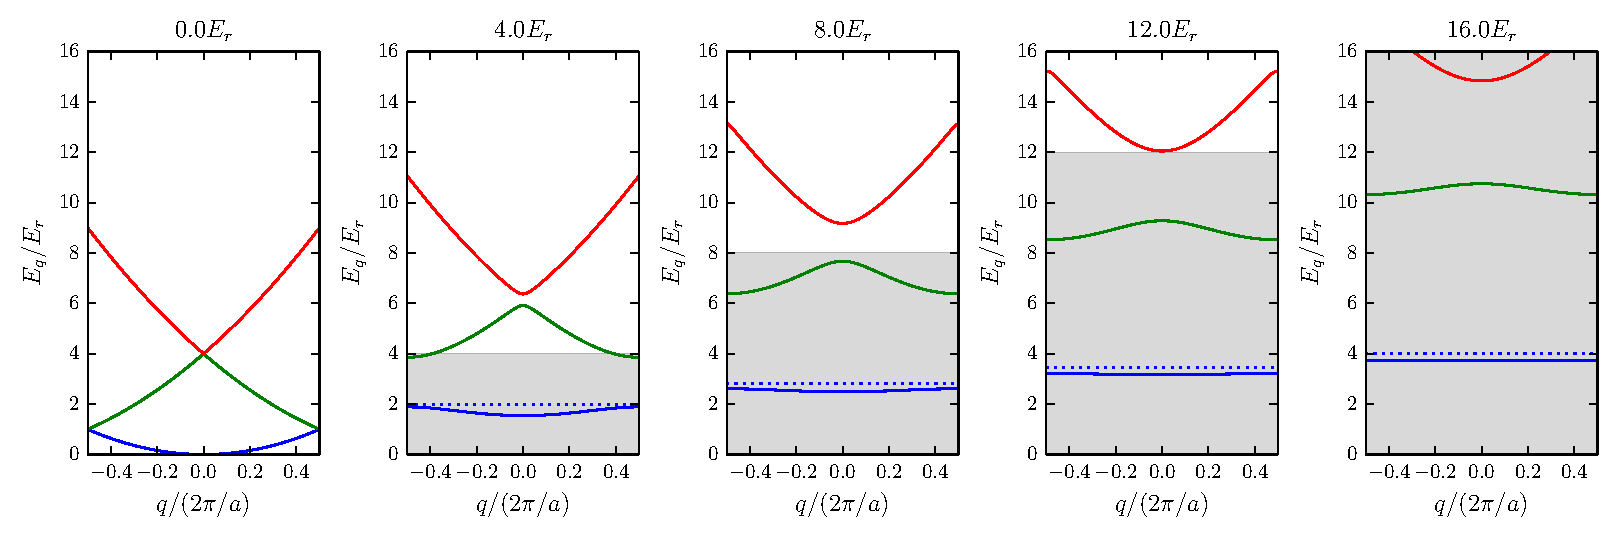
\includegraphics[width=\textwidth]{../figures/BandStructure_figures/bands1d.pdf}
\caption[Band structure in 1D lattice.]{\small Band structure in a 1D optical
lattice.  The depth of the lattice is indicated by the shaded area, and the
energy of the harmonic oscillator ground state in a single lattice site is shown
as a dotted line.  } \label{fig:bands1d}
\end{figure}
\begin{figure}
\centering 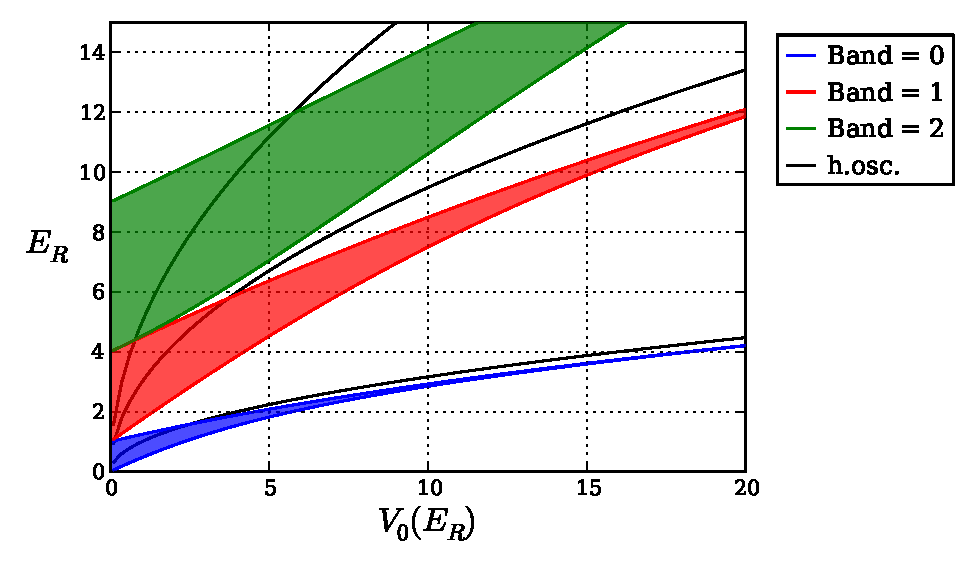
\includegraphics[width=0.6\textwidth]{../figures/BandStructure_figures/bands1d_V0.pdf}
\caption[Band structure in 1D lattice.]{\small Band structure in a 1D optical
lattice.  Each band is indicated by the colored area,  the harmonic oscillator
states in an isolated lattice site are shown as black lines. }
\label{fig:bands1d_V0}
\end{figure}

The time independent Schr\"{o}dinger equation for the hamiltonian in
Eq.~\ref{eq:Hsingle1D}, can also be solved using Mathieu functions.  One can
then calculate the band structure by using the known properties of the Mathieu
functions, which are available on tables or as functions in some software
packages (e.g. Mathematica), see for instance the treatment
in~\cite{PhysRev.87.807}. 

\subsection{Eigenstates}
For each energy eigenvalue we have an associated eigenstate  which is defined
in terms of the $c_{ql}^{n}$ by Eq.~\ref{eq:blochstate}.   Typically, numerical
diagonalization routines return the normalized eigenvectors of the matrix in
question,  and for us this means that the coefficients $c_{ql}^{n}$ will
satisfy
\begin{equation}
   \sum_{l} | c_{ql}^{n} |^{2} = 1 
\end{equation} 
This has the implication that the states obtained from Eq.~\ref{eq:blochstate}
will be normalized over a lattice site.  In Fig.~\ref{fig:eigenfuns1d}. we show
the probability density for a lowest band eigenstate as a function of position
in the lattice for various lattice depths.  One can see how, as the lattice
gets deeper, the state becomes more localized around the center of each lattice
site. 
\begin{figure}
\centering 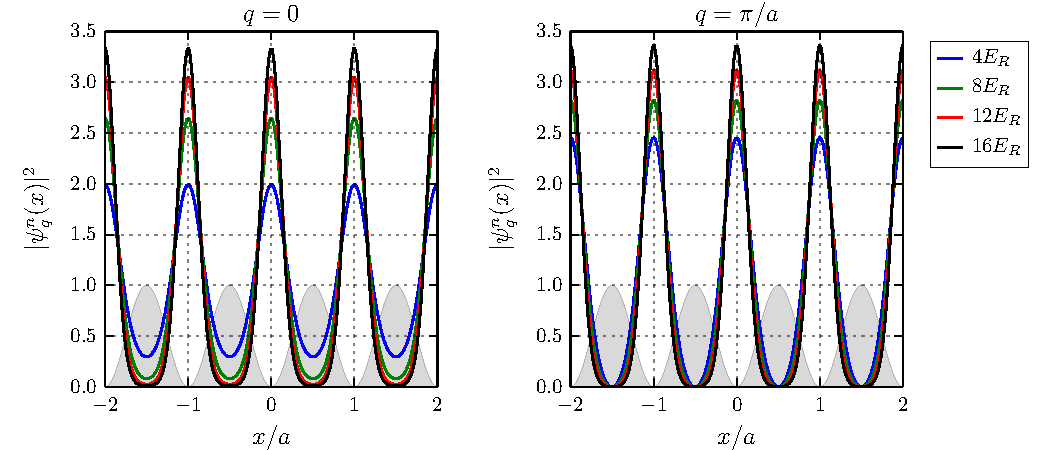
\includegraphics[width=\textwidth]{../figures/BandStructure_figures/eigenfuns1d.pdf}
\caption[Eigenstates in 1D lattice.]{\small Eigenstates of the Hamiltonian in a
1D optical lattice shown for $q=0$ (left) and $q=\pi/a$ (right) for various
lattice depths. The states are normalized so that the integral of the
probability density over one lattice site is equal to one.  The gray shaded
region is shown to indicate the variation of the lattice potential. }
\label{fig:eigenfuns1d}
\end{figure}

\subsection{Wannier states} 
\label{sec:1Dlattice}

It is useful to define a basis of states that are localized around a single
lattice site.  We will see later on that, when using such a basis, the
hamiltonian for the Hubbard model takes its most familiar form.  In a finite
sized lattice with $L$ sites,  the localized state centered around the
$j^{\text{th}}$ site(at $x_{j}$) can be constructed as the following
superposition of eigenstates of the hamiltonian\footnote{In some treatments
(for instance~\cite{salomon2013many}) the Wannier function is defined with a
normalization factor of $\sqrt{L}$  rather than $L$ as shown here.   This is
considering eigenfunctions $\psi_{q}^{n}(x)$ which are normalized when
integrating over the full extent in the lattice.  We stick to the $L$
normalization factor, without the square root, since the eigenfunctions that
are obtained numerically come out normalized over a lattice site, as was
explained in the previous section.}: 
\begin{equation} w^{n}(x-x_{j}) =  \frac{1}{L} \sum_{q}  e^{-i q 2\pi x_{j} }
\psi_{q}^{n}(x) \label{eq:wannier} \end{equation} Here the sum runs over the
set of quasimomenta  $q \in \left\lbrace \frac{2\pi u}{a L} \ |\  u \in \lbrace
0,1,\ldots L-1 \rbrace \right\rbrace$.  Inserting the expansion of
$\psi_{q}^{n}(x)$ in plane waves into the definition of the Wannier state we
obtain 
\begin{equation}
 w^{n}(x-x_{j}) \equiv w_{j}^{n}(x)= 
    \frac{1}{L} \sum_{q}  
   \sum_{l \in \mathbb{Z}} 
   c_{ql}^{n} 
   e^{-i 2\pi q x_{j} }  
   e^{i 2\pi(q+l)x} 
\end{equation}
We will set $x_{j}=0$ for the calculation of the Wannier function,   Wannier
states centered at different lattice sites can be obtained by translation of
the $x_{j}=0$ solution. 
\begin{equation}
  w_{0}^{n}(x)= 
    \frac{1}{L} \sum_{q}  
   \sum_{l \in \mathbb{Z}} 
   c_{ql}^{n} 
   e^{i 2\pi(q+l)x} 
\end{equation}
Since the hamiltonian commutes with the parity operator, it is required that
$\psi_{q}^{n}(-x) = \pm \psi_{q}^{n}(x)$, which implies that $c_{ql}^{n} = \pm
c_{pl'}^{n}$ if  $(q+l) = -(p+l')$.  Using this symmetry, the Wannier state
can be written as 
\begin{equation}
  w_{0}^{n}(x)= 
    \frac{1}{L} \left(
   c_{00}^{n} + 
    \sum_{q>0} 
   \sum_{l > 0 } 
   c_{ql}^{n} \left[ e^{i 2\pi(q+l)x} \pm e^{-i 2\pi(q+l)x } \right] \right)
\end{equation}
It is shown in~\cite{Kohn1959} that the maximally localized Wannier states are
obtained if the plus sign is chosen for even bands and the minus sign is chosen
for odd bands.  So, the $x_{j}=0$ Wannier state is symmetric for the even bands
and antisymmetric for the odd bands.  
\begin{equation}
  w_{0}^{n}(x)= 
    \frac{c_{00}^{n}}{L}
   + 
    \frac{2}{L}
    \sum_{q>0} 
   \sum_{l > 0 } 
   c_{ql}^{n} 
\begin{cases}
\cos[ 2\pi(q+l)x ] & \text{if $n$ even} \\
\sin[ 2\pi(q+l)x ] & \text{if $n$ odd }
\end{cases}
\end{equation}
%For $q,l>0$ all the coefficients $c_{ql}^{n}$ will have the same sign, so we
%select them to be positive.  

After defining the way to construct the Wannier states starting from the
$c_{ql}^{n}$, we can now proceed to add up the plane waves to  obtain the
states, as shown in Fig.~\ref{fig:wannier1d_V0} for various lattice depths.  As
the lattice depth is increased, the Wannier states become more localized, which
leads to less overlap between states in adjacent sites, and results in a
reduction of the probability amplitude for a particle to tunnel from one site
to the neighboring one.   More localized states also imply that the on-site
interaction will be larger, since, on average, two particles in the same site
will be closer to each other.  
\begin{figure}
\centering
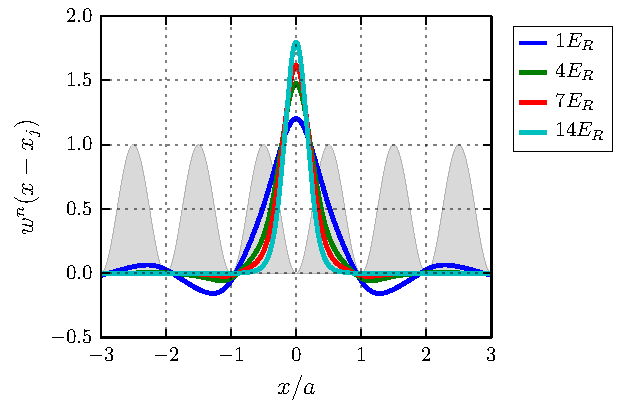
\includegraphics[width=0.6\textwidth]{../figures/BandStructure_figures/wannier1d_V0.pdf}
\caption[Wannier states in 1D lattice for various lattice depths.]{\small
Wannier states localized at $x_{j}=0$ in a 1D optical lattice for various
lattice depths.  The gray shaded region is shown to  indicate the spatial
variation of the lattice potential.  } \label{fig:wannier1d_V0}
\end{figure}

We also show, in Fig.~\ref{fig:wannier1d_bands}, the Wannier functions for the
first three bands in a 4$E_{R}$ lattice.  
\begin{figure}
\centering
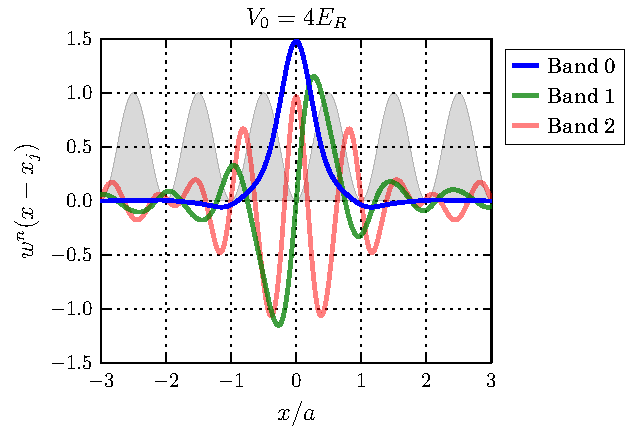
\includegraphics[width=0.6\textwidth]{../figures/BandStructure_figures/wannier1d_bands.pdf}
\caption[Wannier states in 1D lattice for the first three energy bands.]{\small
Wannier states localized at $x_{j}=0$  in a 4$E_{R}$ 1D optical lattice for the
first three energy bands.  The gray shaded region is shown to  indicate the
spatial variation of the lattice potential.  } \label{fig:wannier1d_bands}
\end{figure}

\section{Three-dimensional optical lattice potential}

The hamiltonian for an atom moving in a  3D lattice can be separated in the
three spatial coordinates.  So we can use the solutions that were obtained in
the previous section for the 1D lattice and obtain the band structure and the
Wannier states for the 3D lattice.   The 3D band structure is shown in
Fig.~\ref{fig:bands3d_V0}. 
\begin{figure}
\centering 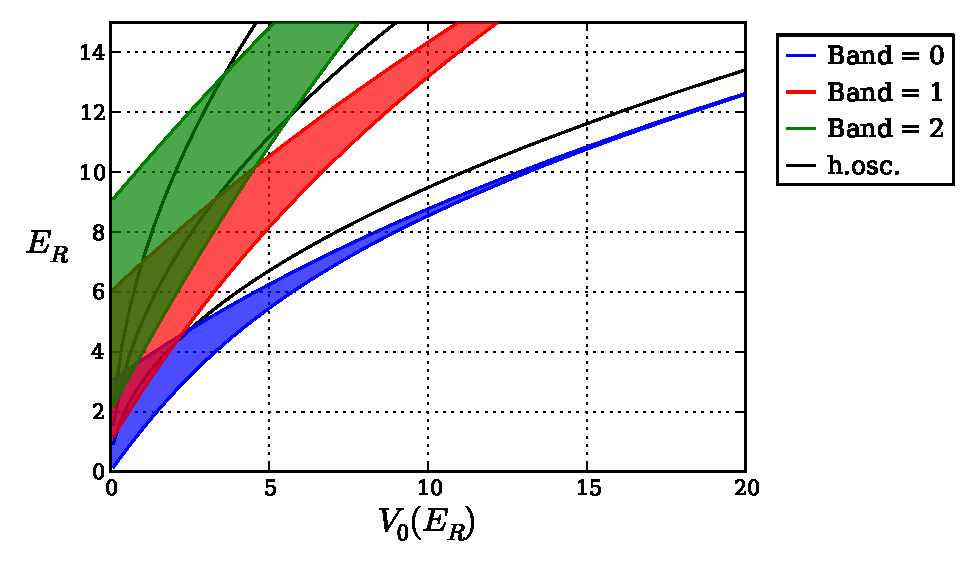
\includegraphics[width=0.6\textwidth]{../figures/BandStructure_figures/bands3d_V0.pdf}
\caption[Band structure in 3D lattice.]{\small Band structure in a 3D optical
lattice.  Each band is indicated by the colored area,  the harmonic oscillator
states in an isolated lattice site are shown as black lines. }
\label{fig:bands3d_V0}
\end{figure}

The Wannier states in a 3D lattice are simply products of the Wannier states in
each of the three spatial coordinates.  They are defined as 
\begin{equation}
 w^{n}(\bv{r}-\bv{r}_{j}) =  \frac{1}{L^{3}} \sum_{\bv{q}} e^{-i \bv{q}\cdot\bv{r}_{j} }
     \prod_{u=x,y,z}  \psi_{q_{u}}^{n_{u}}(u) 
 \label{eq:wannier3D}
\end{equation}
where $L^{3}$ is the total number of sites in the lattice. 

\section{Hubbard hamiltonian}

The many-body Hubbard hamiltonian is 
\begin{equation}
  H =  
-t \sum_{ \langle ij \rangle, \sigma   } 
          a_{i\sigma}^{\dagger}a_{j\sigma} \\
         + U\sum_{i} n_{i\spup} n_{i\spdn}  
\end{equation}
where $i,j$ are indices that run over lattice sites, $\langle ij \rangle$
denotes nearest-neighbors, and $\sigma$ denotes the spin state of the
particles.  The particle creation and annihilation operators,  $a_{j\sigma}$
and $a_{i\sigma}^{\dagger}$,  along with the number operator $n_{i\sigma}$
arise naturally in the second quantization formalism. In what follows, we will
see how to obtain this many-body form, starting from the first quantized
version of the hamiltonian for a system of $N$ particles moving in a periodic
lattice. 


The hamiltonian for a single atom in a 3D optical lattice is given by  
\begin{equation}
  H_{\text{single,3D}} = - \frac{\hbar^{2}}{2m} \left( \frac{\partial^{2}}{\partial x^{2}}
                            + \frac{\partial^{2}}{\partial y^{2}}
                            + \frac{\partial^{2}}{\partial z^{2}} \right)
 + \vo\left( \cos^{2}(kx)  + \cos^{2}(ky) + \cos^{2}(kz) \right)
\end{equation}
and when $N$ particles are considered, along with their interactions the
hamiltonian takes a more complicated form \begin{equation}
\begin{split}
  H = & \sum_{l}^{N}\left[ 
  -\frac{\hbar^{2}}{2m} \left( \frac{\partial^{2}}{\partial x_{l}^{2}}
                            + \frac{\partial^{2}}{\partial y_{l}^{2}}
                            + \frac{\partial^{2}}{\partial z_{l}^{2}} \right)
 + \vo\left( 
        \cos^{2}(kx_{l})  + \cos^{2}(ky_{l}) + \cos^{2}(kz_{l}) 
      \right) \right]\\
      &  + \frac{1}{2}\sum_{ l,n, l\neq n}^{N} 
              V_{\mathrm{int}}(\bv{r}_{l},\bv{r}_{n} )\\ 
    \equiv & ~ H_{0} + H_{\text{int}}
 \label{eq:hubbard1st}
\end{split} 
\end{equation} 
where the particles are labeled by indices $l$,$n$ and $V_{\mathrm{int}}$ is
the potential energy of interaction between two particles.  In the last line we
have defined a more concise notation that splits the Hamiltonian into the
non-interacting ($H_{0}$) and interacting ($H_{\text{int}}$) parts. Solving
this problem is a daunting task primarily for two reasons:
\begin{enumerate}
    \item The Bose or Fermi statistics of the identical particles under
consideration require the solutions to be symmetrized or antisymmetrized
products of single-particle wavefunctions.     
    \item The interactions between the particles prevent a straightforward
reformulation of the problem as a collection of easier-to-solve single particle
hamiltonians.  
\end{enumerate}

The formalism of many-body theory encapsulates a series of methods to deal with
the two issues mentioned above.   First, the reformulation of the Schrodinger
equation in the language of second quantization provides the advantage that the
statistics are automatically taken into account by the notation, so one can
essentially forget about the the (anti)symmetrization of the many-particle wave
functions.  The small price to pay is that one needs to be very careful and
consistent about the order in which operators show up in the notation, since
the symmetry properties of the resulting states are contained in the
commutation relations defined between the operators.  Furthermore, second
quantization makes it easy to consider the extended Hilbert space where the
number of particles is not fixed, known as the Fock space. 

For weak interactions, many-body theory provides a solution to the problem in
terms of perturbation expansions for the physical quantities of interest.   The
theoretical formalism also reduces most of the important physical quantities in
terms of certain matrix elements (Green's functions) which allows the user to
concentrate on obtaining such matrix elements which serve as a starting point
for the exploration of the properties of any system.   The complication arises
when the interactions are not weak, and the perturbative approach of the
many-body formalism breaks down.   


\subsection{Second quantization}

The contents of this section comprise a short summary of the treatment in the
books by Fetter and Walecka~\cite{fetter2003quantum} and
Schwabl~\cite{schwabl2005advanced}.  

Let us start with a complete orthonormal set of single particle states $\lbrace
|i\rangle \rbrace \equiv \lbrace |1\rangle, |2\rangle, \ldots \rbrace$, using these
states we can write the basis states for the $N$-particle system as
\begin{equation}
   | i_{1}, \ldots i_{\alpha}, \ldots i_{N} \rangle \equiv 
   | i_{1}\rangle_{1} \ldots |i_{\alpha}\rangle_{\alpha} \ldots 
   | i_{N} \rangle_{N} ~,
\end{equation} 
which represents a state in which particle 1 is in state $i_{1} \in \lbrace
|i\rangle \rbrace$, particle $\alpha$ is in state $i_{\alpha}$ and so on.
These product states are not eigenstates of the permutation operator $P_{ij}$
which interchanges particles $i$ and $j$.  However, starting from the product
states we can obtain the completely (anti)symmetrized basis states for bosons
(fermions), which are eigenstates of any possible permutation of the
particle labels.  

For bosons, the normalized completely symmetric states are
\begin{equation} 
  | n_{1},  n_{2}, \ldots \rangle = 
  \frac{1}{\sqrt{N!n_{1}!n_{2}!\ldots}} \sum_{P}  
    P | i_{1},  i_{2}, \ldots i_{N} \rangle
\end{equation} 
where the $P$'s are elements of the permutation group\footnote{For $N$
particles there are $N!$ possible permutations and thus $N!$ elements in the
permutation group.}  In this expression, $n_{i}$ is the number of times that
the state $|i\rangle$ occurs among the $N$ particles, also called the
occupation number of state $|i\rangle$.  The sum of all occupation numbers
$n_{i}$ must equal the total number of particles, but otherwise there is no
restriction in the occupation number for bosons.

For fermions the normalized completely antisymmetric states have an extra
factor $(-1)^{P}$, which denotes the parity of the permuatation $P$.  They can
be written in the form of Slater determinants: \begin{equation}
\begin{split}
  | n_{1},  n_{2}, \ldots \rangle = &
  \frac{1}{\sqrt{N!}} \sum_{P} (- 1)^{P} P | i_{1},  i_{2}, \ldots i_{N} \rangle \\
  = &
  \frac{1}{\sqrt{N!}}
  \begin{vmatrix}
  |i_{1}\rangle_{1} & |i_{1}\rangle_{2} & \dotsm & |i_{1}\rangle_{N} \\
  \vdots &  \vdots &  \ddots   & \vdots \\
  |i_{N}\rangle_{1} & |i_{N}\rangle_{2} & \dotsm & |i_{N}\rangle_{N} \\
\end{vmatrix}
\end{split} 
  \label{eq:antisymmetrize} 
\end{equation}  
If a single particle state appears more than once in the product state, the
resulting totally antisymmetric state is zero,  i.e. the occupation numbers
$n_{i}$ can only take the values 0 or 1, a consequence of the Pauli exclusion
principle. 

For bosons (fermions), we can combine the (anti)symmetric states for
$N=0,1,2,\ldots$ particles to obtain a complete orthonormal set of states for
arbitrary particle number.  This ``number states'' are the basis of the Fock
space. 


%We now define the creation  operators for bosons, which allow us to take a
%state from the subspace of $N$ particles, to the subspace of $N+1$  particles.
%\begin{equation}
% a_{i}^{\dagger} | \ldots, n_{i}, \ldots \rangle  = 
% \sqrt{n_{i}+1}|\ldots, n_{i}+1, \dots\rangle
%\end{equation}
%It follows that the adjoint of the creation operator is the annihilation
%operator and satisfies 
%\begin{equation}
%a_{i} | \ldots, n_{i}, \ldots \rangle  
%=\begin{cases}
%\sqrt{n_{i}}|\ldots, n_{i}-1, \dots\rangle
%& \text{if $n_{i}\geq 0$},\\
%0 & \text{if $n_{i}=0$}
%\end{cases}
%\end{equation}
%The creation and annihilation operators are defined such that one can create
%any state starting from the vacuum state $|0\rangle \equiv |0,0,\ldots\rangle$
%in which there are no particles at all.  In more formal terms 
%\begin{equation}
%  | n_{1}, n_{2}, \dots \rangle = \frac{1}{\sqrt{n_{1}!n_{2}!\ldots}} 
%   ( a_{1}^{\dagger} ) ^{n_{1}}  
%   ( a_{2}^{\dagger} ) ^{n_{2}}  \ldots | 0 \rangle
%  \label{eq:numberstate}
%\end{equation}
%The boson creation and annihilation operators satisfty the Bose communtation
%relations 
%\begin{equation}
%  [a_{i}, a_{j}] = 0 \ \ \ \ \  
%  [a_{i}^{\dagger}, a_{j}^{\dagger}] = 0 \ \ \ \ \   
%  [a_{i},a_{j}^{\dagger}]=\delta_{ij}
%\end{equation}

We will concentrate in the case of fermions, and define the creation operators
such that the number state can be written as 
\begin{equation}
 | n_{1}, n_{2}, \ldots \rangle = 
    \left( a_{1}^{\dagger}\right)^{n_{1}} 
    \left( a_{2}^{\dagger}\right)^{n_{2}} \ldots |0\rangle 
%    ~~~~~~ n_{i} = 0\ \text{or}\ 1  
\label{eq:defnumberstate0}
\end{equation}
where $|0\rangle$ is the vacuum state, in which there are no particles.  By
definition, the number state is completely antisymmetric, but what does this
imply for the creation operators?  Going back to Eq.~\ref{eq:antisymmetrize},
which defines the number states,  we see that the sign of the number state
depends on the particular ordering of the single particle states in the Slater
determinant.   Suppose $n_{1}=n_{2}=1$, changing the labels on states 1 and 2
corresponds to exchanging two rows in the Slater determinant and thus a minus
sign comes out: 
\begin{equation} 
    \left( a_{2}^{\dagger}\right)^{n_{2}} 
    \left( a_{1}^{\dagger}\right)^{n_{1}} \ldots |0\rangle  = 
  - | n_{1}, n_{2}, \ldots \rangle 
%    ~~~~~~ n_{i} = 0\ \text{or}\ 1  
\end{equation}
Comparing with Eq.~\ref{eq:defnumberstate0} we notice that the creation
operators must then satisfy the following anticommutation relation
\begin{equation} 
    a_{1}^{\dagger} a_{2}^{\dagger} + a_{2}^{\dagger} a_{1}^{\dagger} 
   \equiv  \left\lbrace  a_{1}^{\dagger} , a_{2}^{\dagger} \right\rbrace 
   = 0 
\end{equation}
Notice that this anticommutation relation implies $\left( a_{i}^{\dagger}
\right)^{2} = 0$, which is yet another manifestation of the Pauli exclusion
principle.
   
When dealing with Fermions, one must decide first on a particular ordering of
the single particle states and then stick to it, noticing that to produce the
number states (without a minus sign) all the creation operators must be applied
to the vacuum state in the chosen order.   The action of a creation operator on
a number state is
\begin{equation}  
  a_{i}^{\dagger}| \ldots, n_{i}, \ldots \rangle 
  =    (-1)^{\sum_{k<i} n_{k}} | \ldots, n_{i}+1, \ldots \rangle 
 \label{eq:defcreation}
\end{equation} 
where the factor $(-1)^{\sum_{k<i} n_{k}}$ takes care of the number of
anticommutations needed to place the $a_{i}^{\dagger}$ operator in the correct
position.  The action of the fermion annihilation operators can be inferred by
taking the adjoint of Eq.~ \ref{eq:defcreation}.  One can then obtain all of
the anticommutation rules for fermions: 
\begin{equation}
  \left\lbrace a_{i}, a_{j} \right\rbrace = 0 \ \ \ \ \  
  \left\lbrace a_{i}^{\dagger}, a_{j}^{\dagger} \right\rbrace = 0 \ \ \ \ \   
  \left\lbrace a_{i},a_{j}^{\dagger} \right\rbrace=\delta_{ij}
\end{equation}


\subsection{Operators in second quantization}

So far two great leaps have been taken: 
\begin{enumerate}
 \item We have swept antisymmetrization under the rug by introducing the number
states, defined from the vacuum in terms of creation operators which satisfy
the Fermi anticommutation rules. 
 
 \item We started from an $N$ particle hamiltonian, but we have now defined
number states that can handle the description of systems with an arbitrary
number of particles 
\end{enumerate}
The two ideas mentioned are related to the states used to describe the system,
now we will turn to the problem of the observables and see how they are handled
in the second quantization.  


Let us consider the sum $\sum_{\alpha} |i\rangle_{\alpha} \langle j | _{\alpha}
$ where $|i\rangle$ and $|j\rangle$ are single particle states, and $\alpha$
runs over all particles in the system.  We apply the sum to the number states
using the definition in Eq.~\ref{eq:antisymmetrize}: 
\begin{equation}
  \left(
   \sum_{\alpha} |i\rangle_{\alpha} \langle j | _{\alpha}  \right)
  | n_{1},  n_{2}, \ldots \rangle = 
  \frac{1}{\sqrt{N!}} \sum_{P} (- 1)^{P} P 
  \left( \sum_{\alpha} |i\rangle_{\alpha} \langle j | _{\alpha} 
   | i_{1},  i_{2}, \ldots i_{N} \rangle \right)
\end{equation}
For the term in the right not to vanish, the initial number state  must have a
particle in state $|j\rangle$, i.e. it must have $n_{j}=1$. Also, $n_{i}$ must
be $n_{i}=0$,  or else the completely antisymmetric state will vanish.  If the
particle initially in state $|j\rangle$ is labeled as  $J$  we can write
\begin{equation}
\begin{split}
  \left(
   \sum_{\alpha} |i\rangle_{\alpha} \langle j | _{\alpha}  \right)
  | n_{1},  n_{2}, \ldots \rangle = &
  \frac{1}{\sqrt{N!}} \sum_{P} (- 1)^{P} P \left( 
    |i_{1}\rangle_{1}
    |i_{2}\rangle_{2}
    \ldots 
     \!\!\!\!\!\!
    \underbrace{ 
    |i\rangle_{J} }_{\text{instead of } |j\rangle_{J}} 
     \!\!\!\!\!\!
    \ldots 
    |i_{N}\rangle_{N}
  \right) \\
   =&  
  \frac{1}{\sqrt{N!}}
  \begin{vmatrix}
  |i_{1}\rangle_{1} & |i_{1}\rangle_{2} & \dotsm & |i_{1}\rangle_{N} \\
  \vdots &  \vdots &     & \vdots \\
  |i\rangle_{1} & |i\rangle_{2} & \dotsm & |i\rangle_{N} \\
  \vdots &  \vdots &     & \vdots \\
  |i_{N}\rangle_{1} & |i_{N}\rangle_{2} & \dotsm & |i_{N}\rangle_{N} \\
\end{vmatrix} \\
\end{split} 
\end{equation}
In the determinant of the left, the state $|i\rangle$ appears in the
$j^{\text{th}}$ row, so a few rows need to be exchanged to put it in the
correct place according to our sign convention for the number states:
\begin{multline}
  \left(
   \sum_{\alpha} |i\rangle_{\alpha} \langle j | _{\alpha}  \right)
  | n_{1},  n_{2}, \ldots \rangle = \\  
 \begin{cases}
(-1)^{\sum_{k<j} n_{k} + \sum_{k<i}n_{k}~~~}
   \,| n_{1}, n_{2},  \ldots, n_{i}+1, \ldots,  n_{j}-1, \ldots  \rangle   
& \text{if $i\leq j$},\\
(-1)^{\sum_{k<j} n_{k} + \sum_{k<i}n_{k} -1 } 
   \,| n_{1}, n_{2},  \ldots, n_{j}-1, \ldots,  n_{i}+1, \ldots  \rangle
& \text{if $i>j$}
\end{cases}  
\end{multline}
Checking the definition of the creation and annihilation operators we obtain
the important result 
\begin{equation}
  \left(
   \sum_{\alpha} |i\rangle_{\alpha} \langle j | _{\alpha}  \right)
  | n_{1},  n_{2}, \ldots \rangle 
   =   a_{i}^{\dagger} a_{j} 
  | n_{1},  n_{2}, \ldots \rangle 
  ~~~~~ \Rightarrow ~~~~~ 
   \sum_{\alpha} |i\rangle_{\alpha} \langle j | _{\alpha} = 
     a_{i}^{\dagger} a_{j} 
\end{equation}

Now, consider an operator $T$ that is a sum over single particle operators
\begin{equation}
  T = \sum_{\alpha} t_{\alpha}
 \label{eq:defsingleparticleop}
\end{equation}  
If we insert the completeness relation for the single particle states twice in
this sum, we have \begin{equation}
\begin{split}
  T = & \sum_{\alpha} \left( \sum_{i} |i\rangle_{\alpha}\langle i |_{\alpha} \right)
        t_{\alpha} \left( \sum_{j} |j\rangle_{\alpha}\langle j |_{\alpha} \right) \\
    = & \sum_{ij}   \langle i | t | j \rangle  \sum_{\alpha} |i\rangle_{\alpha} \langle j |_{\alpha} \\ 
    = & \sum_{ij}   \langle i | t | j \rangle a_{i}^{\dagger} a_{j} \equiv \sum_{ij} t_{ij}   a_{i}^{\dagger} a_{j} 
\end{split}  
\end{equation}
This is the other big leap provided by the second quantization:  an operator
that was written as a sum over particles becomes a sum of creation and
annihilation operators.   We will apply this prescription to the
non-interacting part of the Hamiltonian for $N$ particles moving in a lattice.  

Operators like the potential energy, which are a sum over two-particle (or
many-particle) operators,  can be similarly expressed as sums of creation and
annihilation operators~\cite{schwabl2005advanced}.  For a two-body operator we
have the expression
\begin{equation}
\begin{split}
F = & \frac{1}{2} \sum_{\alpha\neq\beta} f(\bv{r}_{\alpha}, \bv{r}_{\beta} )  \\
  = & \frac{1}{2} \sum_{ijkm} \langle ij | f | km \rangle 
        a_{i}^{\dagger} a_{j}^{\dagger} a_{m} a_{k} 
\end{split}
\end{equation}

\subsection{Second quantized Hubbard hamiltonian}

The Hubbard hamiltonian in Eq.~\ref{eq:hubbard1st} is a sum of two
single-particle operators and one two-particle operator.  These are,
respectively: the kinetic energy, the energy of the atoms in the lattice
potential, and the interactions between the atoms.  In this section we will
express the Hubbard hamiltonian in second quantized form.  As a single-particle
basis we will use the Wannier states that were derived in
Section.~\ref{sec:1Dlattice}

%In the Hubbard hamiltonian the two single-particle operators are grouped
%together to define the non-interacting part of the hamiltonian 
%\begin{equation}
%\begin{split}
%  H_{0} = & \sum_{l}^{N} -\frac{\hbar^{2}}{2m} \left( \frac{\partial^{2}}{\partial x_{l}^{2}}
%                            + \frac{\partial^{2}}{\partial y_{l}^{2}}
%                            + \frac{\partial^{2}}{\partial z_{l}^{2}} \right)
% + \vo\left( \cos^{2}(kx_{l})  + \cos^{2}(ky_{l}) + \cos^{2}(kz_{l}) \right) \\
%       = & \sum_{l}^{N} H_{\text{single,3D}}^{l}
%\end{split}
%\end{equation}

\paragraph{Tunneling matrix element, $\bm{t}$.} $H_{0}$ is a single particle
operator of the kind defined in Eq.~\ref{eq:defsingleparticleop}:
\begin{equation}
  H_{0} = 
     \sum_{l=1}^{N} H_{\text{single,3D}}^{l}
\end{equation}
where 
\begin{equation}
H_{\text{single,3D}}^{l} = 
  -\frac{\hbar^{2}}{2m} \left( \frac{\partial^{2}}{\partial x_{l}^{2}}
                            + \frac{\partial^{2}}{\partial y_{l}^{2}}
                            + \frac{\partial^{2}}{\partial z_{l}^{2}} \right)
 + \vo\left( \cos^{2}(kx_{l})  + \cos^{2}(ky_{l}) + \cos^{2}(kz_{l}) \right) 
\end{equation}
It's second quantized form it can be written as 
\begin{equation}
\begin{split}
  H_{0} = & \sum_{ij} \langle i| H_{\text{single,3D}} |j \rangle a_{i}^{\dagger} a_{j} \\
        \equiv & ~ -\sum_{ij} t_{ij}  a_{i}^{\dagger} a_{j} \\
\end{split}
\end{equation}  
Note that the sign of $t_{ij}$ was picked rather arbitrarily to follow the
usual conventions.  We now proceed to find the value of the matrix element
$t_{ij}$.  We use the definition of the Wannier states given in
Eq.~\ref{eq:wannier3D} to find 
\begin{equation}
\begin{split}
-t_{ij}  
= & 
  \frac{1}{L^{6}}\int \mathrm{d}\bv{r}\ 
     \sum_{\bv{q}'} e^{i \bv{q'}\cdot\bv{r}_{i} }
     \prod_{u'=x,y,z}  \psi_{q'_{u'}}^{n'_{u'}*}(u') 
  \Big( H_{\text{single,3D}}  \Big)
     \sum_{\bv{q}} e^{-i \bv{q}\cdot\bv{r}_{j} }
     \prod_{u=x,y,z}  \psi_{q_{u}}^{n_{u}}(u)\\ 
= &
  \sum_{\bv{q}\bv{q}'}   
  \frac{E_{\bv{q}}^{n}}{L^{6}}
   e^{ i \bv{q}'\cdot\bv{r}_{i} }  e^{ -i \bv{q}\cdot\bv{r}_{j} }
   \int\mathrm{d}\bv{r}\ 
     \prod_{u'=x,y,z}  \psi_{q'_{u'}}^{n'_{u'}*}(u') 
     \prod_{u=x,y,z}  \psi_{q_{u}}^{n_{u}}(u) \\ 
= &
  \sum_{\bv{q}\bv{q}'}   
  \frac{E_{\bv{q}}^{n}}{L^{6}}
   e^{ i \bv{q}'\cdot\bv{r}_{i} }  e^{ -i \bv{q}\cdot\bv{r}_{j} }
   \delta_{\bv{q}\bv{q}'} \delta_{nn'} L^{3} \\
= &
  \frac{1}{L^{3}}
  \sum_{\bv{q}}   E_{\bv{q}}^{n}
   e^{ i \bv{q}\cdot(\bv{r}_{i} - \bv{r}_{j}) } \\
\end{split} 
\end{equation}
We observe that there is no amplitude to go between states that are in two
different bands, as is indicated by the appearance of $\delta_{nn'}$.   In what
follows, we will consider only the lowest band, $n=0$,  so we will drop the
band index altogether.  This simplification imposes two important requirements
for our system:
 
\begin{enumerate}
\item \textbf{The temperature and the Fermi energy need to be small compared to
the energy gap between the lowest and first excited band.}

\item \textbf{The interaction energy scale must also be small compared to the
energy gap between the lowest and first excited band.}
\end{enumerate}

In the 3D lattice, the total energy $E_{\bv{q}}$ is the sum of the energy
associated with each quasimomentum component, $E_{\bv{q}} = \sum_{u=x,y,z}
E_{q_{u}} $.  By inserting this into the sum for $t_{ij}$ above we find 
\begin{multline}
-t_{ij} =  \frac{1}{L^{3}} \left[ 
          \left(\sum_{q_{x}} E_{q_{x}}   e^{ i q_{x} x_{ij} }   \right)
          \sum_{q_{y}} e^{ i q_{y} y_{ij} }   
          \sum_{q_{z}} e^{ i q_{z} z_{ij} }  
   \right. \\
\left. 
          + 
          \sum_{q_{x}} e^{ i q_{x} x_{ij} }  
          \left(\sum_{q_{y}} E_{q_{y}}   e^{ i q_{y} x_{ij} }   \right)
          \sum_{q_{z}} e^{ i q_{z} z_{ij} }  
          + 
          \sum_{q_{x}} e^{ i q_{x} x_{ij} }  
          \sum_{q_{y}} e^{ i q_{y} y_{ij} }   
          \left(\sum_{q_{z}} E_{q_{z}}   e^{ i q_{z} z_{ij} }   \right)
\right]
\end{multline}
We make use of the identity $\sum_{q_{u}} e^{ iq_{u}(u_{i}-u_{j}) } = L \delta_{u_{i}u_{j}}$ to obtain
\begin{equation}
-t_{ij} =  \frac{1}{L} \left[ 
          \left(\sum_{q_{x}} E_{q_{x}}^{\text{\tiny 1D}}   e^{ i q_{x} x_{ij} }   \right)
          \delta_{y_{i}y_{j}}
          \delta_{z_{i}z_{j}}
          + 
          \left(\sum_{q_{y}} E_{q_{y}}^{\text{\tiny 1D}}   e^{ i q_{y} x_{ij} }   \right)
          \delta_{x_{i}x_{j}}
          \delta_{z_{i}z_{j}}
          + 
          \left(\sum_{q_{z}} E_{q_{z}}^{\text{\tiny 1D}}   e^{ i q_{z} z_{ij} }   \right)
          \delta_{x_{i}x_{j}}
          \delta_{y_{i}y_{j}}
\right]
\label{eq:tunnelinglong}
\end{equation}

If $i=j$ we have 
\begin{equation}
  -t_{ii} =  \frac{3}{L} 
          \sum_{q} E_{q} 
\end{equation}
Since $q$ runs over the $L$ different values in the set $q \in \left\lbrace
\frac{2\pi u}{a L} \ |\  u \in \lbrace 0,1,\ldots L-1 \rbrace \right\rbrace$,
$-t_{ii}$ is nothing more than the mean energy of the 3D energy band, which we will refer to as $E_{0}$,  $-t_{ii}\equiv E_{0}$  

If $i\neq j$,  tunneling can only occur along one of the lattice directions as
can be seen from the different Kronecker delta terms that show up in
Eq.~\ref{eq:tunnelinglong}.   In other words, for the simple cubic potential,
diagonal tunneling events are second order processes.  If we write the distance
between sites $i$,$j$ as $\Delta_{ij}$, the tunneling matrix element simplifies
to  \footnote{In this section we have used the Wannier states constructed as a
sum of plane waves to obtain the tunneling matrix element.  It can also be
obtained directly from the Wannier states'  wavefunctions:
\begin{equation}
  -t_{ij} = \int \mathrm{d}\bv{r} \, w_{i}(\bv{r}) H_{\text{single,3D}} w_{j}(\bv{r}) 
\end{equation}
Calculating the tunneling matrix element by computing the overlap integral of
the Wannier wavefunctions is computationally more expensive than obtaining it as
a sum over the energy eigenvalues. }
\begin{equation}
  -t_{ij} = \frac{1}{L} \sum_{q} E_{q} e^{iq \Delta_{ij}} 
\label{eq:tunneling3D}
\end{equation}
In the tight-binding approximation, terms for which $|\Delta_{ij}|>a$ are
neglected, and  $\Delta_{ij}$ can only take the values $-a$ or $a$,
where $a$ is the lattice spacing.  In this case we use $t_{ij}\equiv t$, where
$t$ is given by
\begin{equation}
  -t = \frac{1}{L} \sum_{q} E_{q} e^{iqa} 
\label{eq:tunneling3D_tight}
\end{equation}

We can then go ahead and write the second quantized form of $H_{0}$ in the
tight-binding approximation 
\begin{equation} 
  H_{0}  =  E_{0} \sum_{i}  a_{i}^{\dagger} a_{i}  - t 
    \sum_{ \langle i j \rangle }
                      a_{i}^{\dagger} a_{j}   
\end{equation} 
The first term in this expression is constant for a system with a conserved
number of particles, since $\sum_{i}  a_{i}^{\dagger} a_{i}=N$.    Usually this
energy offset is neglected, but when dealing with inhomogeneous systems which
have a position dependent lattice depth it will be important to take it into
account, as we will see later on.   


We can go ahead and invert the Fourier series in Eq.~\ref{eq:tunneling3D} to
obtain 
\begin{equation} 
  E_{q} = - \sum_{\Delta_{ij}} t_{ij} e^{-iq \Delta_{ij}} 
\end{equation}
which in the tight-binding approximation reduces to 
\begin{equation}
  E_{q} = -2 t\cos( qa) 
\end{equation}
This explicit form for the dispersion relation allows us to relate the
bandwidth, $W_{\text{1D}}$, to the tunneling matrix element as
$W_{\text{1D}}=4t$,  which in 3D becomes $W_{\text{3D}}= 12t$.

It is useful to find out the range of lattice depths for which the
tight-binding approximation is valid in the optical lattice potential.  To do
this we just need to look at the tunneling matrix elements for beyond
nearest-neighbor tunneling,  as shown in Fig.~\ref{fig:tightbinding}.  For
lattice depths $\gtrsim 5 E_{R}$  we can safely ignore beyond nearest-neighbor
tunneling, see also Fig.~\ref{fig:hubbardvalid}.  
\begin{figure}
\centering
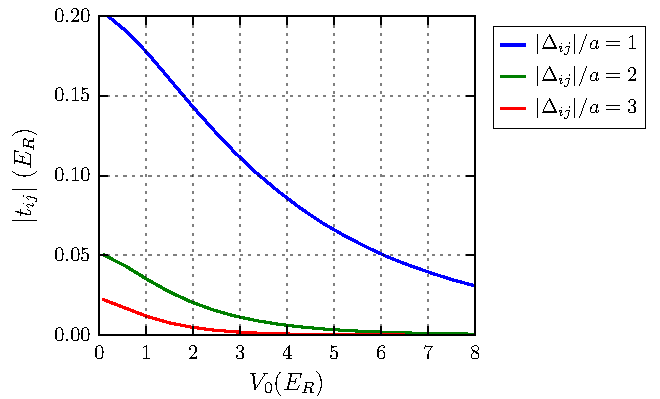
\includegraphics[width=0.6\textwidth]{../figures/BandStructure_figures/tightbinding_V0_interp.pdf}
\caption[Tunneling matrix elements in a 3D lattice.]{\small Tunneling matrix
element in an optical lattice as a function of lattice depth.  Nearest-neighbor
and beyond nearest-neighbor matrix elements are shown to illustrate the range
of lattice depths for which the tight-binding limit is a good approximation.
$\Delta_{ij}$ corresponds to the distance between initial and final lattice
sites in the tunneling matrix element.  } \label{fig:tightbinding}
\end{figure}

Yet another way of estimating the tunneling matrix element \cite{Bloch2008} is
by using the relationship $t=W_{\text{1D}}/4$, valid in the tight-binding
limit,  and obtaining the bandwidth from the known properties of the Mathieu
functions, which are solutions to the Schrodinger equation in a 1D lattice.
This yields the analytic result 
\begin{equation}
 t/\er \simeq \frac{4}{\sqrt{\pi}} \vvo^{3/4} \exp(-2\sqrt{\vvo}) 
\label{eq:tunnelMathieu}
\end{equation} 
where \vvo\ is the lattice depth in units of the recoil energy. The comparison
between the result from Eq.~\ref{eq:tunneling3D} and Eq.~\ref{eq:tunnelMathieu}
is shown in Fig.~\ref{fig:tMathieu}. 
\begin{figure}
\centering
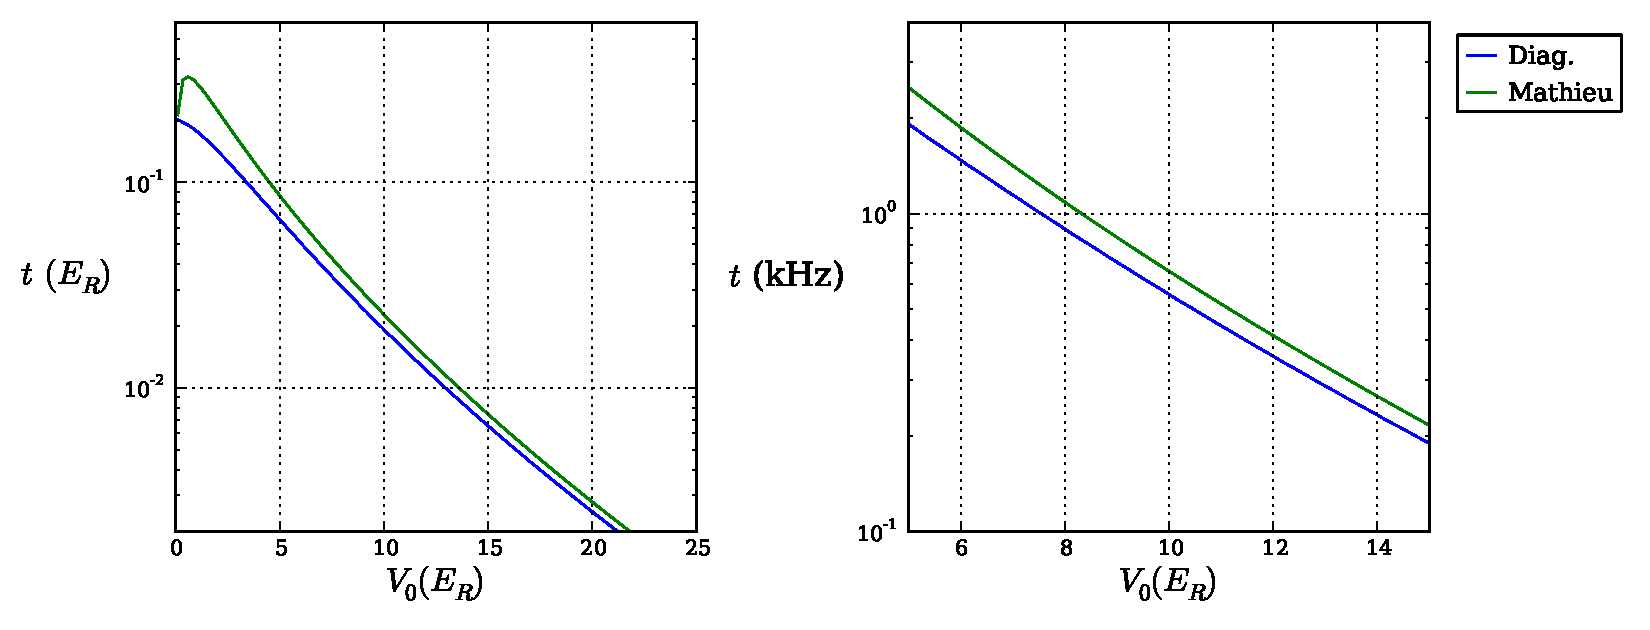
\includegraphics[width=\textwidth]{../figures/BandStructure_figures/tunneling_V0_Mathieu.pdf}
\caption[Nearest neighbor tunneling matrix element]{\small Nearest neighbor
tunneling matrix element in an optical lattice as a function of lattice depth.
Comparison between the result from Eq.~\ref{eq:tunneling3D} and the one
obtained from the Mathieu functions, Eq.~\ref{eq:tunnelMathieu}.  The right
panel shows the tunneling rate in kHz for the mass of a $^{6}$Li atom.  }
\label{fig:tMathieu}
\end{figure}

%Finally, we have the second quantized form of $H_{0}$ in the tight-binding
%limit 
%\begin{equation}
%  H_{0} = -t \sum_{ \langle ij \rangle } a_{i}^{\dagger}a_{j} 
%\end{equation}
%where the $\langle \rangle$ denote nearest-neighbors, and the creation operator
%$a_{i}^{\dagger}$ create particles in the Wannier state localized at site $i$.

Notice that, up to now, we have ignored the spin part of the wavefunction.   We
can include it easily by noticing that $H_{0}$ does not act on the spin at
all, so the states $|i\rangle$ and $|j\rangle$ that we have used in the
derivation above need to have the same spin.   If two spin states are
available, our basis set is twice as large, which can be taken care of by
including a sum over spin states:
\begin{equation}
  H_{0} = E_{0}N\, -\ t
   \!\!\! 
  \sum_{ \langle ij \rangle, \sigma=\dbl   } 
   \!\!\!
  a_{i\sigma}^{\dagger}a_{j\sigma} 
\end{equation}

\paragraph{On-site interaction energy, $\bm{U}$.}

The interaction part of the hamiltonian for $N$ particles is
given by \begin{equation}
    H_{\text{int}} = 
         \frac{1}{2}\sum_{ l,m, l\neq m}^{N} 
         V_{\mathrm{int}}(\bv{r}_{l},\bv{r}_{m} )\\ 
\end{equation}
This is a two-particle operator, and its second quantized form is given by
\begin{equation}
   H_{\text{int}} = \frac{1}{2} \sum_{i,j,k,m} 
           \langle ij | V_{\mathrm{int}} | km \rangle
           a_{i}^{\dagger} a_{j}^{\dagger} a_{m} a_{k}
\end{equation}
where 
\begin{equation}
    \langle ij | V_{\mathrm{int}} | km \rangle =
    \int \mathrm{d}\bv{r}_{1} \int \mathrm{d}\bv{r}_{2} \ \  
    \varphi_{i}^{*}(\bv{r}_{1}) \varphi_{j}^{*}(\bv{r}_{2}) 
    V_{\mathrm{int}}(\bv{r}_{1},\bv{r}_{2}) 
    \varphi_{k}(\bv{r}_{1}) \varphi_{m}(\bv{r}_{2}) 
\end{equation}
and the $\varphi$'s correspond to the wavefunctions of the single particle
basis states chosen. 

The interaction between ultracold atoms can be described in terms of the
$s$-wave scattering length, $a_{s}$,  and a
pseudo-potential~\cite{sakurai2014modern,Bloch2008} given by\footnote{This is a
good approximation as long as the $s$-wave scattering lengths is small compared
to the single-site harmonic oscillator length~\cite{Busch1998}. This condition
is typically satisfied, and other concerns such as collisional losses or
coupling to higher bands are significant before the $s$-wave scattering length
becomes comparable to the harmonic oscillator length.  The harmonic oscillator
length in a lattice site is $\ell = a / (\pi \vvo^{1/4})$, which for a 7\,\er\
lattice with $a=532\,$nm is $\ell \approx 2000\,a_{0}$, where $a_{0}$ is the
Bohr radius.}
\begin{equation}
    V_{\mathrm{int}}(\bv{r}_{1},\bv{r}_{2}) 
    = \frac{ 4 \pi \hbar^{2} a_{s} } { m } \delta(\bv{r}_{1}-\bv{r}_{2}) 
\end{equation}
so the matrix element above can be written as 
\begin{equation}
    \langle ij | V_{\mathrm{int}} | km \rangle =
\frac{ 4 \pi \hbar^{2} a_{s} } { m }
    \int \mathrm{d}\bv{r}  \ \  \varphi_{i}^{*}(\bv{r}) \varphi_{j}^{*}(\bv{r}) \varphi_{k}(\bv{r}) \varphi_{m}(\bv{r}) 
\end{equation}
Our basis states, $\varphi$, are the 3D Wannier states defined in
Eq.~\ref{eq:wannier3D}, which are separable in the three spatial coordinates.
We recall that the Wannier states are labeled by the lattice site around which
they are centered, and by their band index.   If we explicitly write out the two
labels in the expression above, we obtain
\begin{equation}
    \langle ij | V_{\mathrm{int}} | km \rangle =
\frac{ 4 \pi \hbar^{2} a } { m }
  \prod_{v=x,y,z}
    \int \mathrm{d}v  \ \ 
    w_{i}^{n_{i}}(v) w_{j}^{n_{j}}(v) w_{k}^{n_{k}}(v) w_{m}^{n_{m}}(v) 
   \equiv \, U_{ijkm}
\end{equation}

In general $i,j,k,m$ can represent any lattice sites.  We will restrict
our treatment to on-site interactions by enforcing $i=j=k=m$,  furthermore, we
consider only Wannier states in the lowest band. 
%The Wannier function along  $x,y,z$ depends on the lattice depth along the
%respective coordinate.  We will consider a lattice with different depths along
%the three spatial coordinates, $\bvo = ( V_{0x}, V_{0y}, V_{0z} ) $.  At this
%point we make the approximation of neglecting all of the off-site interaction
%terms, which can be justified by the localized nature of the Wannier states.
%Furthermore, we consider only Wannier states in the lowest band, which is
%valid for scattering lengths smaller than the single-site harmonic oscillator
%length~\cite{Busch1998}.  
With this considerations, and also explicitly writing down the spin quantum
number, which so far was implicit in the indices $ijkm$, we find 
\begin{equation}
   H_{\text{int}} =  
           \frac{U}{2}\sum_{\sigma\neq\sigma'}\sum_{i} 
           a_{i\sigma}^{\dagger} a_{i\sigma'}^{\dagger} a_{i\sigma'} a_{i\sigma} \\
\end{equation}
where we have defined $U\equiv U_{ijkm}$ for $i=j=k=m$. 
Within the single band approximation to the on-site interactions, we have  
%\begin{equation}
%  U = 
%  \frac{ 4 \pi \hbar^{2} a } { m }
%   \prod_{v=x,y,z}  \int  w(v) ^{4} \mathrm{d}v  
%\end{equation}
%In units of $E_{R}$, 
\begin{equation}
  U/\er = \frac{ 8}{ \pi}  \frac{ a_{s} }{a}
   \prod_{v=x,y,z}  \int  w(v) ^{4} \mathrm{d}v  
\end{equation}

Defining the number operator as $n_{i\sigma} = a_{i\sigma}^{\dagger}
a_{i\sigma}$ 
\begin{equation}
\begin{split}
   H_{\text{int}}  
     = & \  
           \frac{U}{2}\sum_{\sigma\neq\sigma'}\sum_{i}
           n_{i\sigma'} n_{i\sigma}  \\
     = & \ 
           U\sum_{i}
           n_{i\spup} n_{i\spdn}  
\end{split}
\end{equation}
where $i$ runs over all of the lattice sites.  


To calculate the value of $U$ we use the Wannier states obtained in
Sec.~\ref{sec:1Dlattice}.  Alternatively, one can approximate the Wannier state
by the Gaussian ground state in the local oscillator potential of one lattice
site and carry out the integral analytically to obtain~\cite{Bloch2008} 
\begin{equation} 
  U  = \sqrt{ 8\pi } \frac{a_{s}}{a} \vvo^{3/4} 
\end{equation} 
Figure~\ref{fig:wfactor} shows a comparison of the exact result and the
Gaussian approximation to the Wannier state for a lattice with
$\lambda=1064$\,nm. 
\begin{figure}
\centering
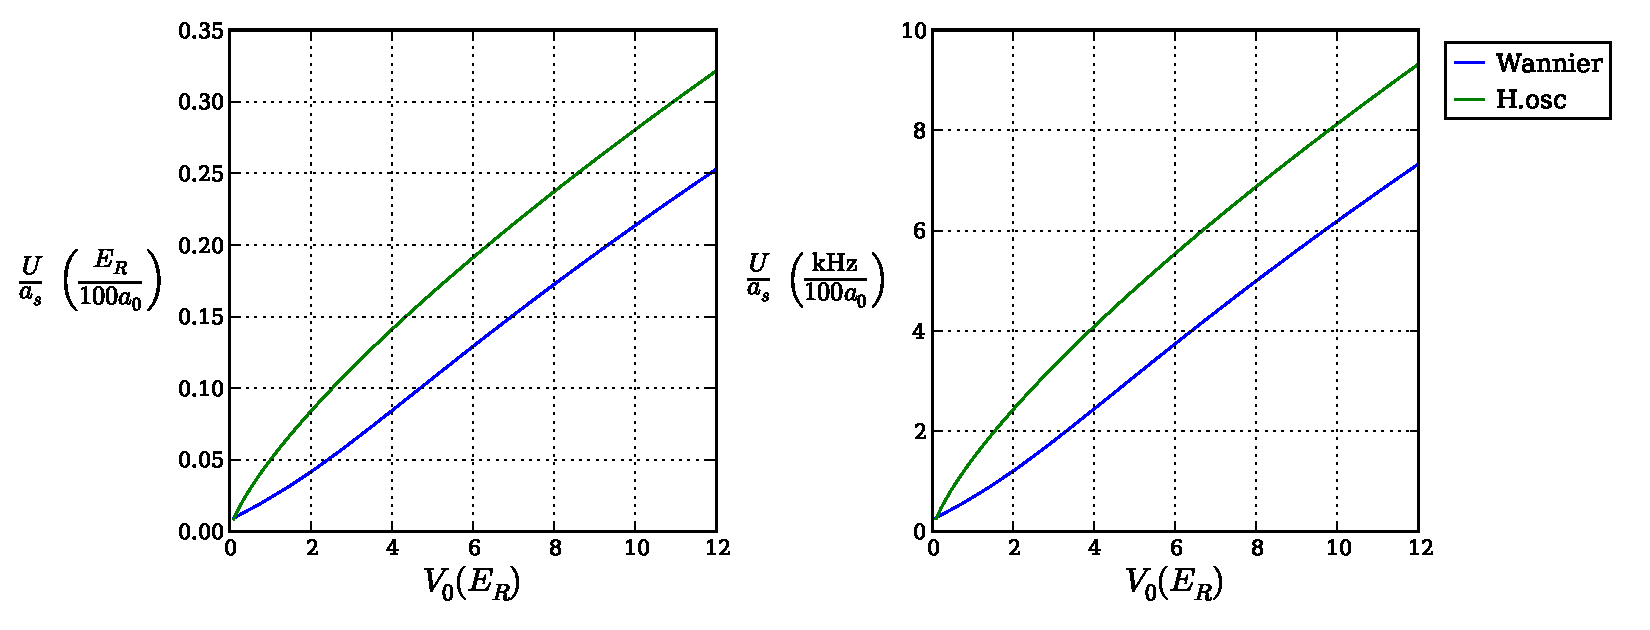
\includegraphics[width=\textwidth]{../figures/BandStructure_figures/wFactor_V0_a0.pdf}
\caption[On-site interactions in a 3D lattice]{\small On-site interactions in a
3D lattice ($\lambda=1064\,\text{nm}$) as a function of lattice depth.
Numerical calculation using Wannier functions compared to the approximation
using harmonic oscillator states.  The lattice depth is the same in all three
directions of the lattice.   The left panel shows uses \er\ for the units of $U$ 
and the right panel uses kHz for $U/h$. }
\label{fig:wfactor}
\end{figure}

If the on-site interaction term is comparable to the energy spacing between the
lowest and first excited bands, the single band approximation presented here
breaks down.  Corrections to the tunneling rate and the on-site interactions
are necessary, which may depend on the lattice site
occupation~\cite{Werner2005,Jordens2010,Mark2012}.

\section{Parameter regimes for a valid description using a single band
Hubbard model}

Throughout this chapter we have mentioned the possible scenarios for which the
single band Hubbard model is not an accurate description of ultracold atoms in
an optical lattice.  The two most important ones are:
\begin{itemize} 
\item The on-site interaction $U$ is comparable to the band gap $\Delta$.  The
band gap is the energy difference between the highest energy state in the
lowest band and the lowest energy state in the first excited band, see
Fig.~\ref{fig:bands3d_V0}. \item Tunneling beyond nearest-neighbor (rate
$t_{2}\equiv t_{ij}$ for $\Delta_{ij}=2a$, see Fig.~\ref{fig:tightbinding}) is
not negligible compared to nearest-neighbor tunneling (rate $t$), i.e.  the
tight-binding approximation does not hold. 
\end{itemize}
In Fig.~\ref{fig:hubbardvalid} we have represented these two conditions as a
function of the lattice depth and the $s$-wave scattering length.  For more
details on the validity of the single band Hubbard hamiltonian see
Ref.~\cite{Werner2005}. 
\begin{figure}
\centering
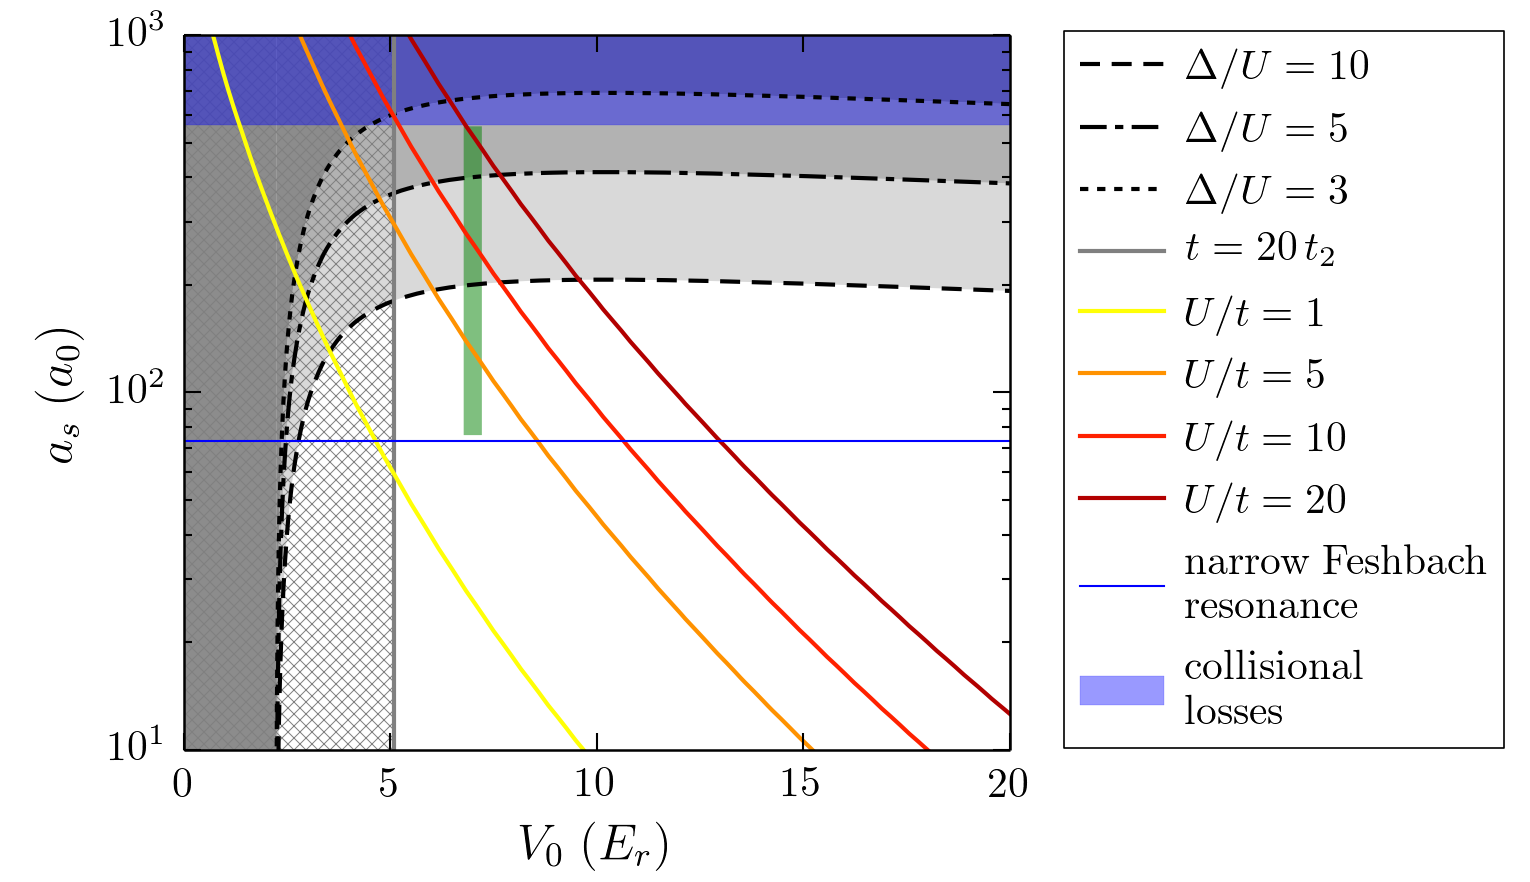
\includegraphics[width=0.9\textwidth]{../figures/BandStructure_figures/singleband.png}
\caption[Regimes of validity for the single band Hubbard hamiltonian]{\small
Regimes of validity for the single band Hubbard hamiltonian.   The dashed black
lines show curves at constant $\Delta/U$.  As $U$ approaches $\Delta$, higher
bands have to be taken into account to describe the system
accurately~\cite{Werner2005}.  The vertical gray line indicates the lattice
depth at which $t = 20t_{2}$, which delimits the region of validity of the
tight-binding approximation.  Yellow to brown hued lines indicated curves at
constant $U/t$.  The thin blue line indicates the background $s$-wave
scattering length in the vicinity of the narrow Feshbach resonance of
$^{6}Li$~\cite{Strecker2003,Zurn2013}.  The shaded blue area indicates the
range of scattering lengths over which we see significant collisional losses
and heating of the sample.   The shaded green area denotes the parameter regime
covered by the experiments carried out in this thesis.} 
\label{fig:hubbardvalid}
\end{figure}


 
%%%%%%%%%%%%%%%%%%%%%%%%%%%%%%%%%%%%%%%%%%%%%%%%%%%%%%%%%%%%%%%%%%%%%%%%%%%%%%%
%%%%%%%%%%%%%%%%%%%%%%%%%%%%%%%%%%%%%%%%%%%%%%%%%%%%%%%%%%%%%%%%%%%%%%%%%%%%%%%
%%%%  CHAPTER 3 
%%%%%%%%%%%%%%%%%%%%%%%%%%%%%%%%%%%%%%%%%%%%%%%%%%%%%%%%%%%%%%%%%%%%%%%%%%%%%%%
%%%%%%%%%%%%%%%%%%%%%%%%%%%%%%%%%%%%%%%%%%%%%%%%%%%%%%%%%%%%%%%%%%%%%%%%%%%%%%%
\chapter{The Hubbard model}

Approximate solutions to the Hubbard model are explained,  including the
high-temperature series expansion (HTSE) which is widely used throughout this
thesis.   

%The Fermi-Hubbard model was formally presented to the world by Hubbard in his
%1950 paper titled ``whatever''.  Perhaps he could suspect at the time that he
%was then fathering a model that to this day remains at the center of condensed
%matter physics.   

%In this section I present the model in its original context, as a
%simplification of the description of valence electrons in crystalline solids.
%I include some historical background to motivate the reader.  
%
%Models for electrons existed which explained conduction phenomena in a
%successful manner.  Also, models existed which dealt with magnetic phenomena.
%This section touches on the necessity to formulate a model that could
%incorporate both transport and magnetic properties of a material.   This need
%arises due to the existence of materials that are at neither end of the
%spectrum.  That is, metals or insulators for which magnetic effects played an
%important role.   The simple example being MnO, on which antiferromagnetism was
%first observed,  and the big challenge being high-temperature
%superconductors. 

\section{Simplified treatments}

This section explains our understanding of the Fermi-Hubbard model.  It starts
by building some insight by using the results of exactly solvable models.   The
results of exact diagonalization in systems of 2-sites and 4-sites are shown.
This are going to motivate the antiferromagnetic character of the ground state,
while showing that there is always a bit of an admixture of double occupancy in
the exact ground state.  

The 4-site solution can be used to help understand why the Fermi-Hubbard is
relevant to high-Tc superconductors.   In this case one can make connections to
the $d$-wave character of ground states upon doping the system.   

The exact diagonalization solutions are at zero temperature, so they give most
insight to the exact ground states of the system. 

\subsection{ Exact diagonalization } 
\subsubsection { 2 site exact diagonalization } 
\subsubsection { 4 site plaquette an relevance to high-Tc superconductors}

\subsection{ Limiting cases} 

This section deals with the limiting cases of the Fermi-Hubbard parameters.
The solutions that are obtained give insights to the workings of the model.
The high temperature series expansion is introduced, which is very relevant for
calculating thermodynamic quantities in the temperature regime of a few times
$T_{\mathrm{Neel}}$.  

\subsubsection { U=0 limit, t=0 limit }


\section{ High-temperature series expansion } I will explain the derivation and
results of the high temperature series expansion to second order in $T/t$. 

\section{ Modern techniques }
In this section I plant to give an outline of DQMC and NLCE. 
%%%%
%%%%In the atomic limit, where tunneling between sites is neglected completely, the
%%%%Hubbard model can solved exactly.  In this case the tunneling part of the
%%%%hamiltonian can be treated as a perturbation and we can gain insight in to the
%%%%different phases that the system can exhibit.  This Section follows the
%%%%treatment that can be found in~\cite{Henderson1992,Jordens2010}.   
%%%%
%%%%We work in the grand canonical ensemble, so we include a global chemical potential
%%%%in the hamiltonian
%%%%\begin{equation}
%%%%\begin{split}
%%%%  H = &  
%%%%         \left( U\sum_{i} n_{i\spup} n_{i\spdn}  
%%%%         - \mu\sum_{i}( n_{i\spup} + n_{i\spdn} ) \right)
%%%%-t \sum_{ \langle ij \rangle, \sigma   } 
%%%%          a_{i\sigma}^{\dagger}a_{j\sigma} \\
%%%%   = &  H_{0} + H_{1} 
%%%%\end{split}
%%%%\end{equation}
%%%%For the unperturbed part, $H_{0}$, the grand canonical partition function is 
%%%%\begin{equation}
%%%% Z_{0} = \text{Tr} e^{-\beta H_{0}} 
%%%%\end{equation}
%%%%Since the unperturbed part is a sum over sites, the partition function becomes
%%%%a product of the single site partition function, $Z_{0} = z_{0}^{k}$, for a
%%%%system with $k$ sites.  The single site partition function  is easy to
%%%%calculate because the trace runs over the only four possible states in a single
%%%%site $\lbrace |0\rangle, |\spup\rangle, |\spdn\rangle, |\dbl\rangle\rbrace$.
%%%%\begin{equation}
%%%% z_{0} = 1 + 2 e^{\beta\mu} + e^{\beta (2\mu-U)} = 1 + 2z + z^{2}u 
%%%%\end{equation}
%%%%where we have defined $z=e^{\beta\mu}$ and $u=e^{-\beta U }$.  Among the
%%%%relevant physical quantities that can be obtained are the number of particles,
%%%%the number of double occupancies, and the entropy per site.  These are obtained
%%%%from the first derivatives of the grand canonical potential, $\Omega$
%%%%\begin{equation}
%%%%  \Omega = - \frac{\ln Z}{\beta}
%%%%\end{equation}
%%%%\begin{gather}
%%%%  N = -\frac{\partial \Omega}{ \partial \mu }\\
%%%%  D = \frac{\partial \Omega}{ \partial U }  \\
%%%%  S = -\frac{\partial \Omega}{ \partial T} 
%%%%\end{gather}
%%%%%\begin{gather}
%%%%%  N = -\frac{\partial \Omega}{ \partial \mu }  = z \frac{\partial}{\partial z} \ln Z\\
%%%%%  D = \frac{\partial \Omega}{ \partial U }  = u \frac{\partial}{\partial u} \ln Z\\
%%%%%  S = -\frac{\partial \Omega}{ \partial T}  = -\beta^{2}  \frac{\partial}{\partial \beta} \ln Z
%%%%%\end{gather}
%%%%Also, from the second derivatives of the grand potential one can obtain the
%%%%fluctuations in any of these quantities. 
%%%%
%%%%For the full hamiltonian the grand canonical partition function $Z$ can be
%%%%expanded in a perturbation series~\cite{Henderson1992} 
%%%%\begin{equation}
%%%%\begin{split}
%%%%  Z = & \text{Tr} e^{-\beta H}  \\
%%%%    = & Z_{0} \left[ 1 + 
%%%%        \sum_{n=1}^{\infty} (-1)^{n} 
%%%%        \int_{0}^{\beta} d\tau_{1} \int_{0}^{\tau_{1}} d\tau_{2} 
%%%%        \dotsm \int_{0}^{\tau_{n-1}} d\tau_{n} 
%%%%        \langle
%%%%              \tilde{H}_{1}(\tau_{1}) 
%%%%              \tilde{H}_{2}(\tau_{2})  \dotsm
%%%%              \tilde{H}_{n}(\tau_{n})  \rangle 
%%%%              \right] 
%%%%\end{split}
%%%%\end{equation} 
%%%%where the thermal expectation value is taken with the
%%%%unperturbed part of the hamiltonian
%%%%\begin{equation}
%%%%\langle A \rangle = \text{Tr} ( e^{\beta H_{0} } A ) / Z_{0} 
%%%%\end{equation}
%%%%and the tilde means that the operator is evaluated in the interaction picture
%%%%for the imaginary time in parenthesis: 
%%%%\begin{equation}
%%%% \tilde{H}_{1}(\tau) = e^{\tau H_{0}} H_{1} e^{-\tau H_{0}} 
%%%%\end{equation}
%%%%Given the series expansion for $Z$, the grand potential is 
%%%%\begin{equation}
%%%% -\beta \Omega = Z_{0} + 
%%%%        \sum_{n=1}^{\infty} (-1)^{n} 
%%%%        \int_{0}^{\beta} d\tau_{1} \int_{0}^{\tau_{1}} d\tau_{2} 
%%%%        \dotsm \int_{0}^{\tau_{n-1}} d\tau_{n} 
%%%%        \langle
%%%%              \tilde{H}_{1}(\tau_{1}) 
%%%%              \tilde{H}_{2}(\tau_{2})  \dotsm
%%%%              \tilde{H}_{n}(\tau_{n})  \rangle 
%%%%\end{equation}
%%%%
%%%%One can see that the $n^{th}$ term in the expansion has $n$ copies of the
%%%%tunneling part of the hamiltonian.  Each  application of $H_{1}$ in the thermal
%%%%average results in a particle tunneling to a neighboring site, so we see that
%%%%there will be a contribution to the expansion only if after $n$ tunneling
%%%%events all the particles come back to their original sites.  A direct
%%%%consequence of this is that the first order term in the expansion vanishes.
%%%%The second order in the expansion corresponds to particles tunneling one site
%%%%over and then coming back.  Higher order terms can be represented by diagrams,
%%%%to make them easier to keep track off.  The contribution from orders up to
%%%%$n=9$ is shown in~\cite{Henderson1992}.  Here we will use up to the second
%%%%order term to illustrate the phases that appear in the system.  
%%%%
%%%%The grand potential to second order is~\cite{Henderson1992,Jordens2010} 
%%%%\begin{equation}
%%%%-\beta \Omega_{2} = k \ln z_{0} + k \left( \frac{\beta t }{z_{0}} \right)^{2} m 
%%%%        \left( z + z^{3} u + 2z^{2} \frac{1-u}{\beta U} \right) 
%%%%\end{equation} 
%%%%where $m$ is the number of nearest neighbors for each lattice site, which in
%%%%the simple cubic case is $m=6$.  We see that the grand potential is
%%%%proportional to the number of lattice sites, so we will obtain all the
%%%%thermodynamic quantities per lattice site. 
%%%%
%%%%The resulting phase diagram is shown in Fig.~\ref{fig:highTphases}.  NOTE FOR
%%%%GROUP MEETING:  I intend to write some text that discusses the relevant phases
%%%%in this phase diagram.  I will discuss them in the presentation in the group
%%%%meeting and add the explanatory text in this document later on.  
%%%%\begin{figure}
%%%%\centering 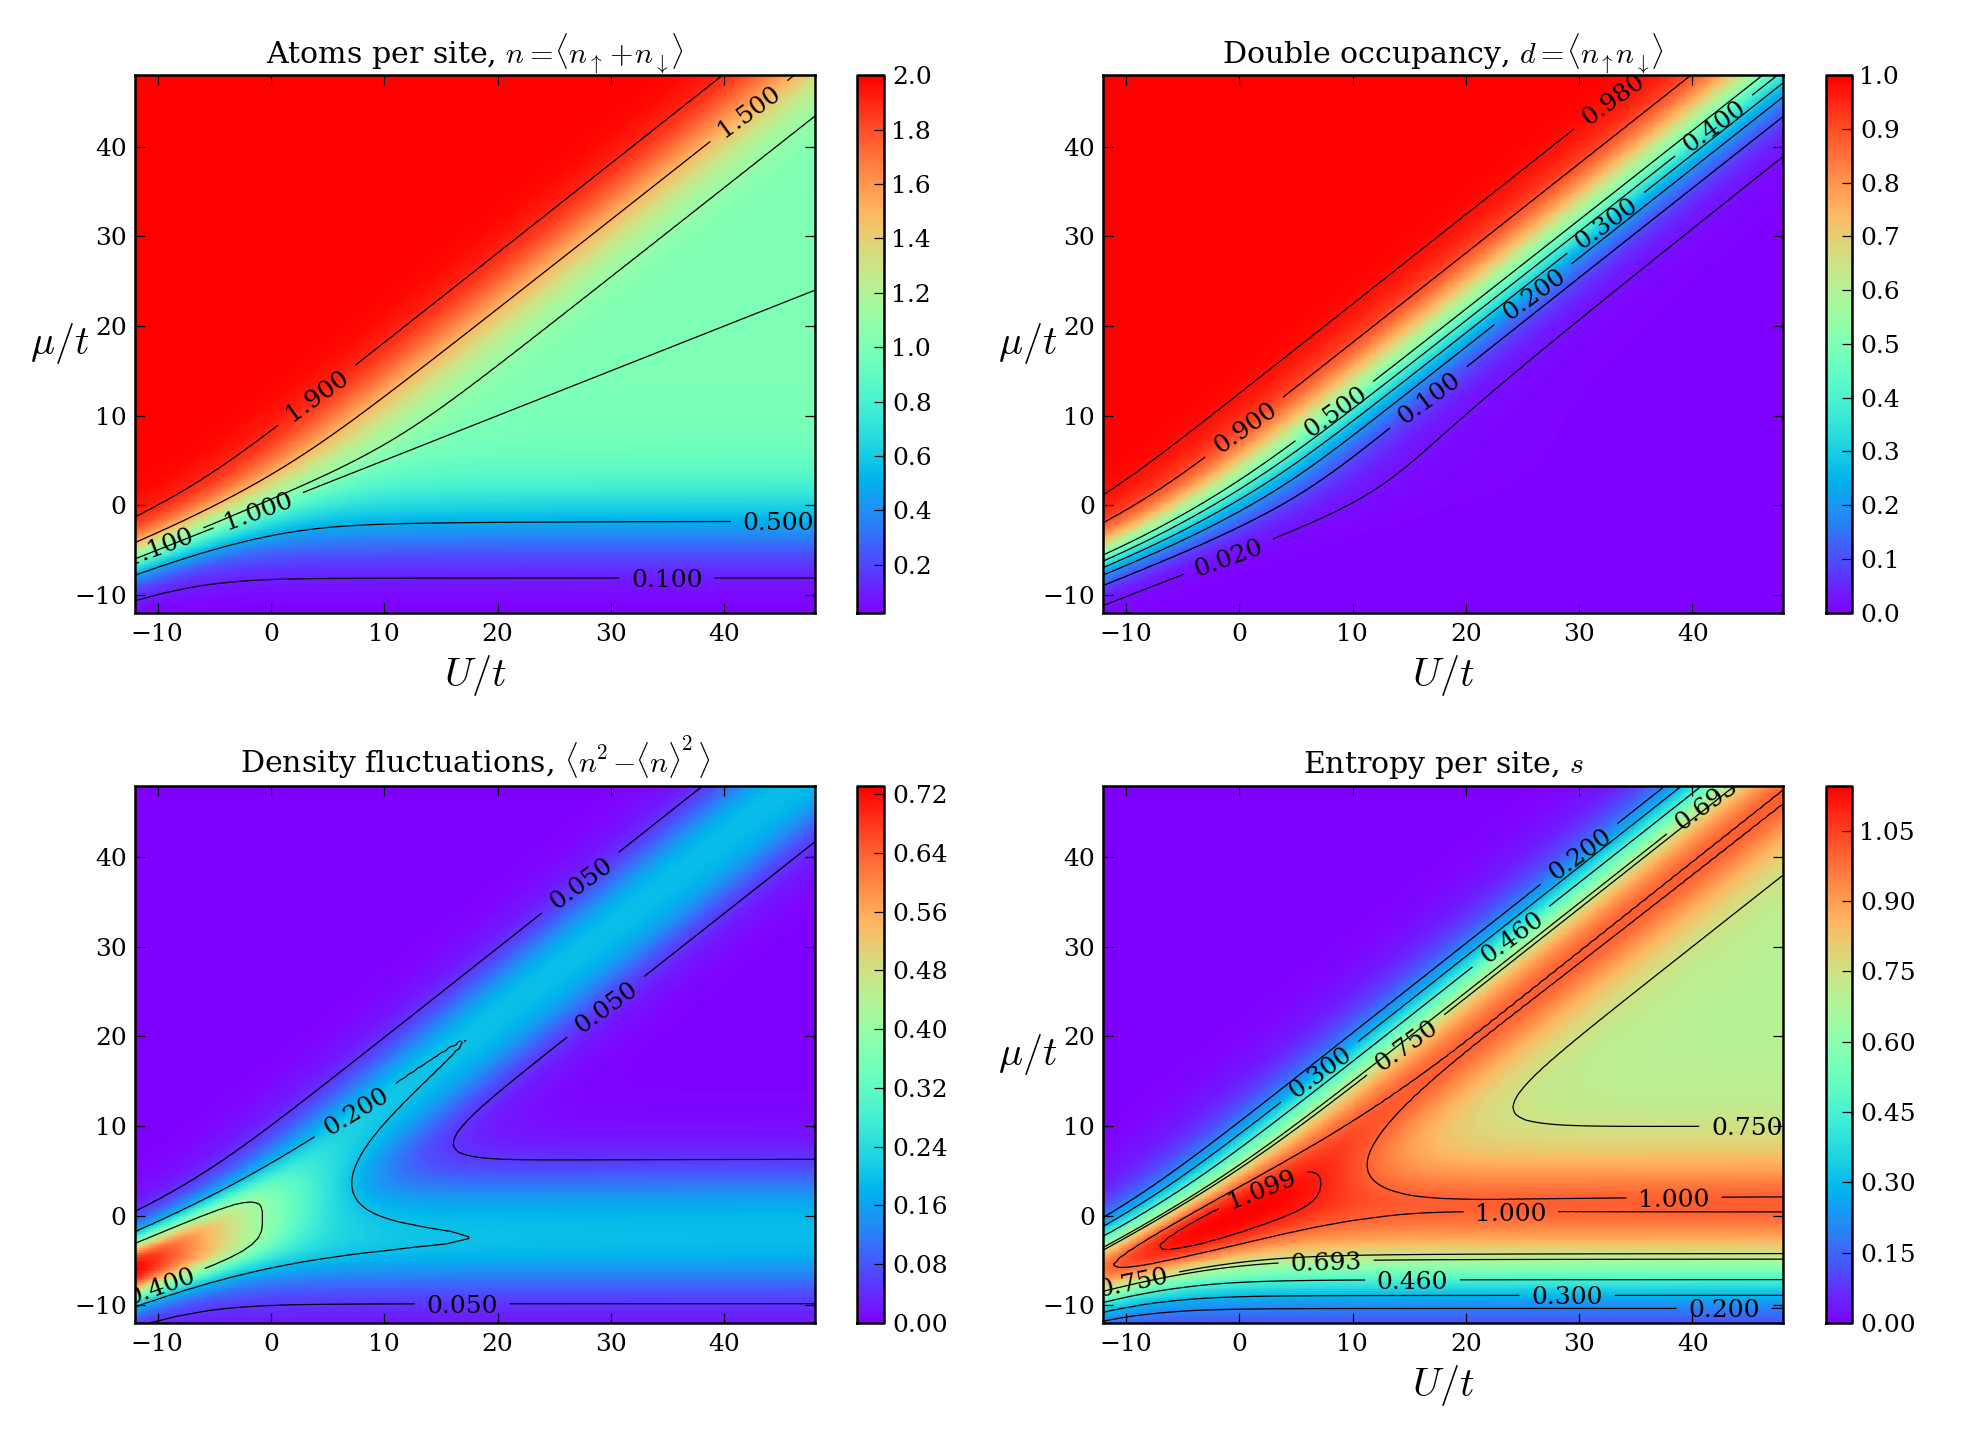
\includegraphics[width=\textwidth]{../figures/HubbardPhaseDiagram_figures/HTSE_phasesT025.png}
%%%%\caption[High temperature phase diagram of the Fermi-Hubbard model]{\small 
%%%%High temperature phase diagram of the Fermi-Hubbard model calculated using only the second order in the perturbation series. 
%%%%} \label{fig:highTphases}
%%%%\end{figure}
%%%%
%%%%\subsubsection{Thermodynamics at colder temperatures, approach to the N\'{e}el transition}
%%%%
%%%%In this section we show the phase diagram for the Fermi-Hubbard model at lower
%%%%temperatures, which are beyond the scope of the perturbation expansion shown in
%%%%the previous section.   The phase diagram was calculated in~\cite{Fuchs2011} by
%%%%using cluster dynamical mean-field theory, and they have made their results
%%%%available in the supplementary material accompanying their paper.  In
%%%%Figures~\ref{fig:fuchs10},\ref{fig:fuchs01},\ref{fig:fuchs03} we show the
%%%%resulting phase diagram for $T/t=$ 10, 1, and 0.3 respectively.
%%%%
%%%%\begin{figure}
%%%%\centering 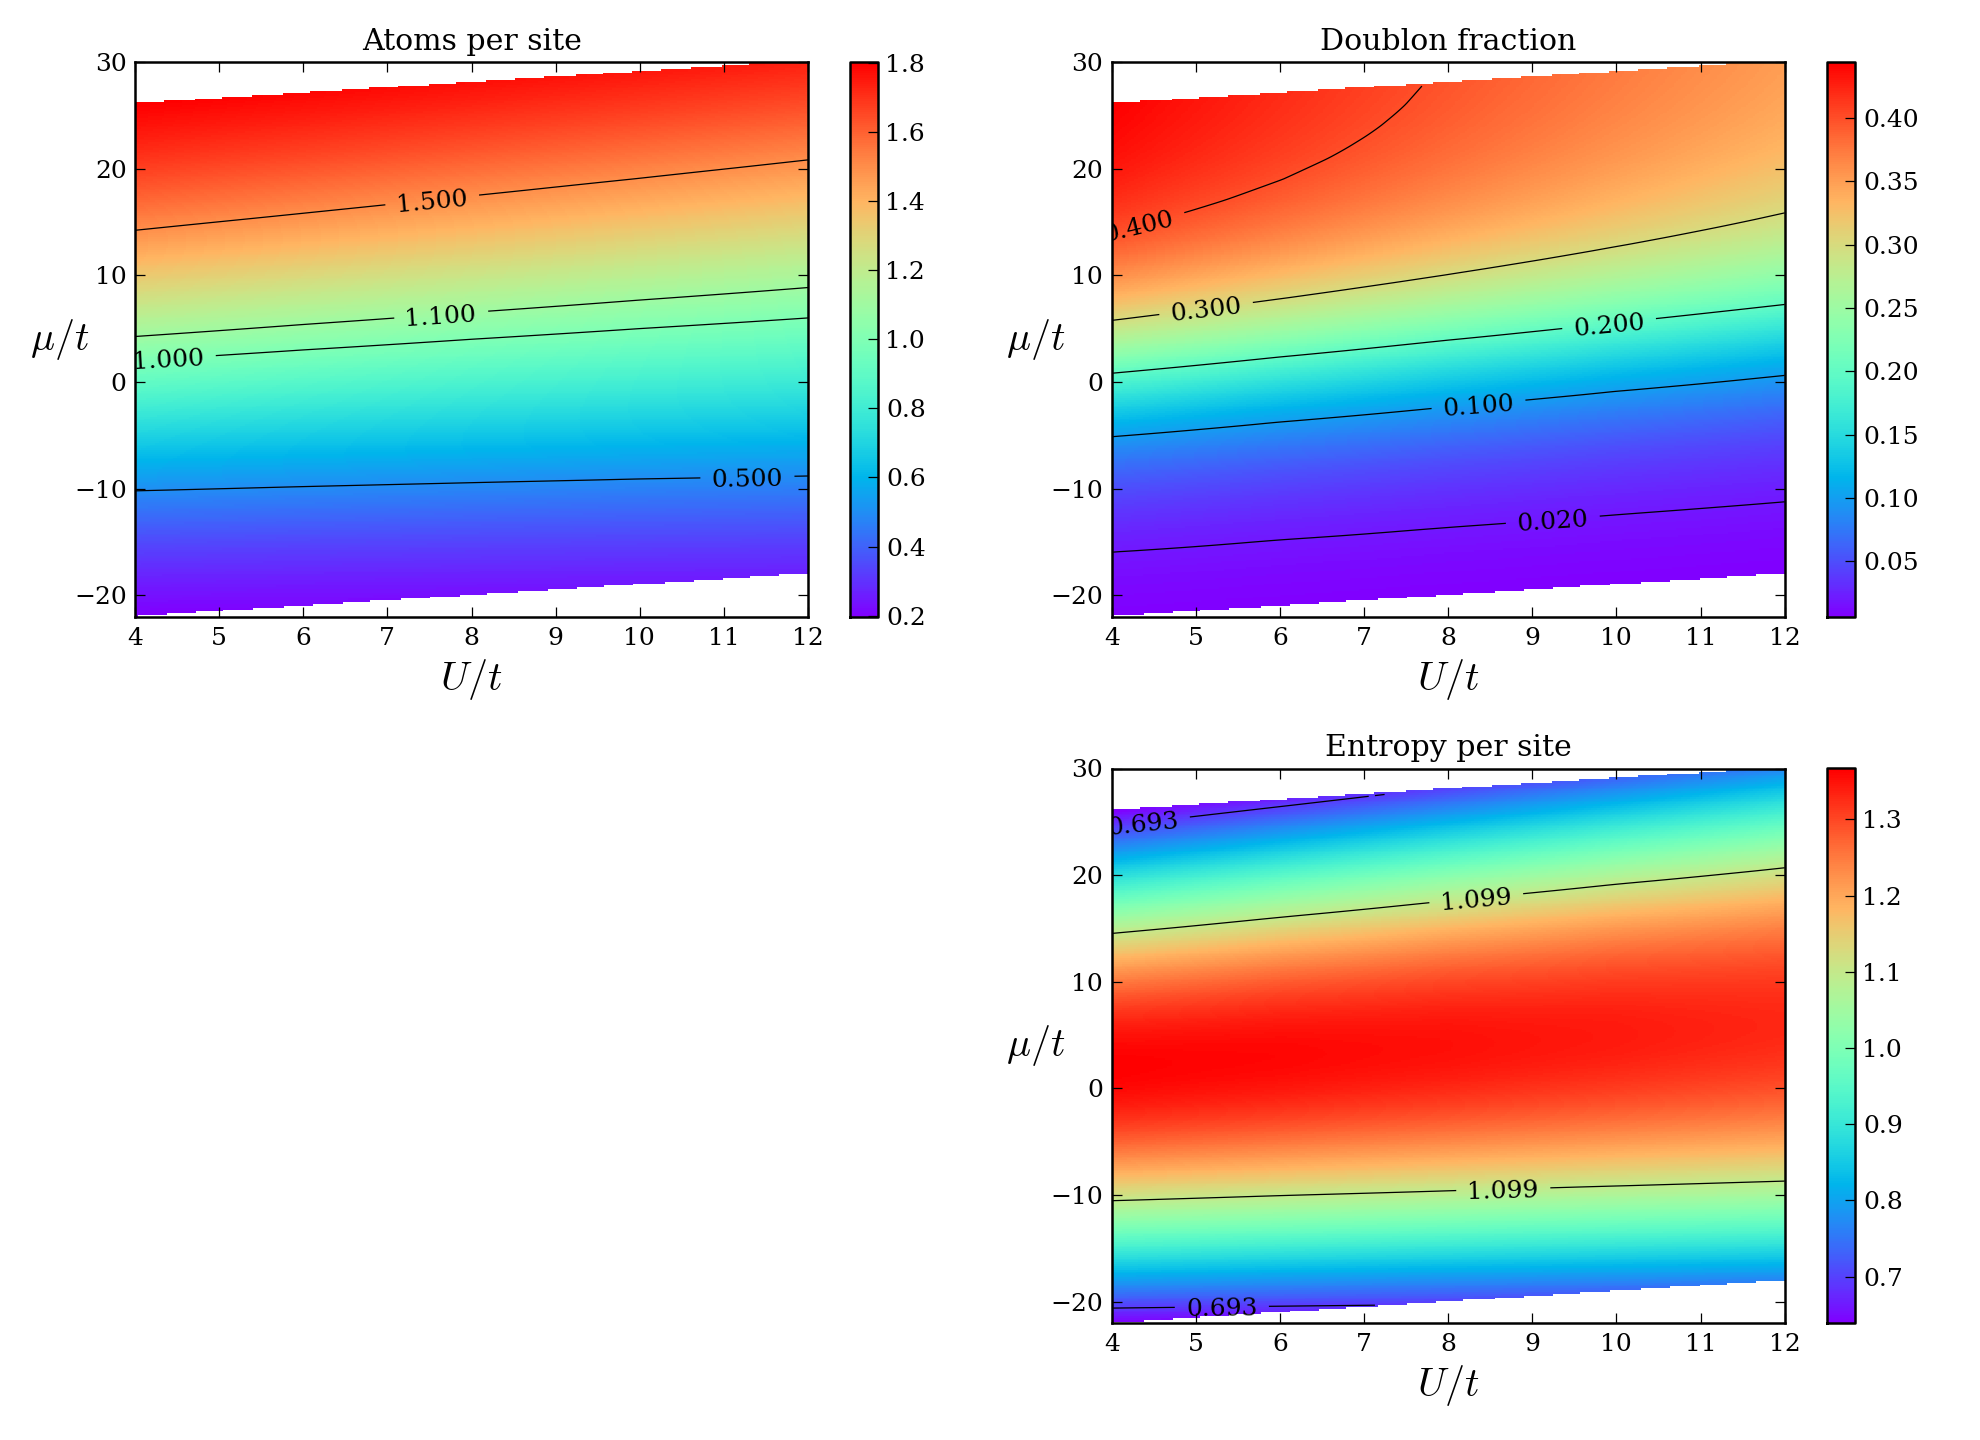
\includegraphics[width=\textwidth]{../figures/HubbardPhaseDiagram_figures/FUCHS_phasesT=100.png}
%%%%\caption[Low temperature phase diagram of the Fermi-Hubbard model]{\small
%%%%From~\cite{Fuchs2011}} \label{fig:fuchs10}
%%%%\end{figure}
%%%%
%%%%\begin{figure}
%%%%\centering 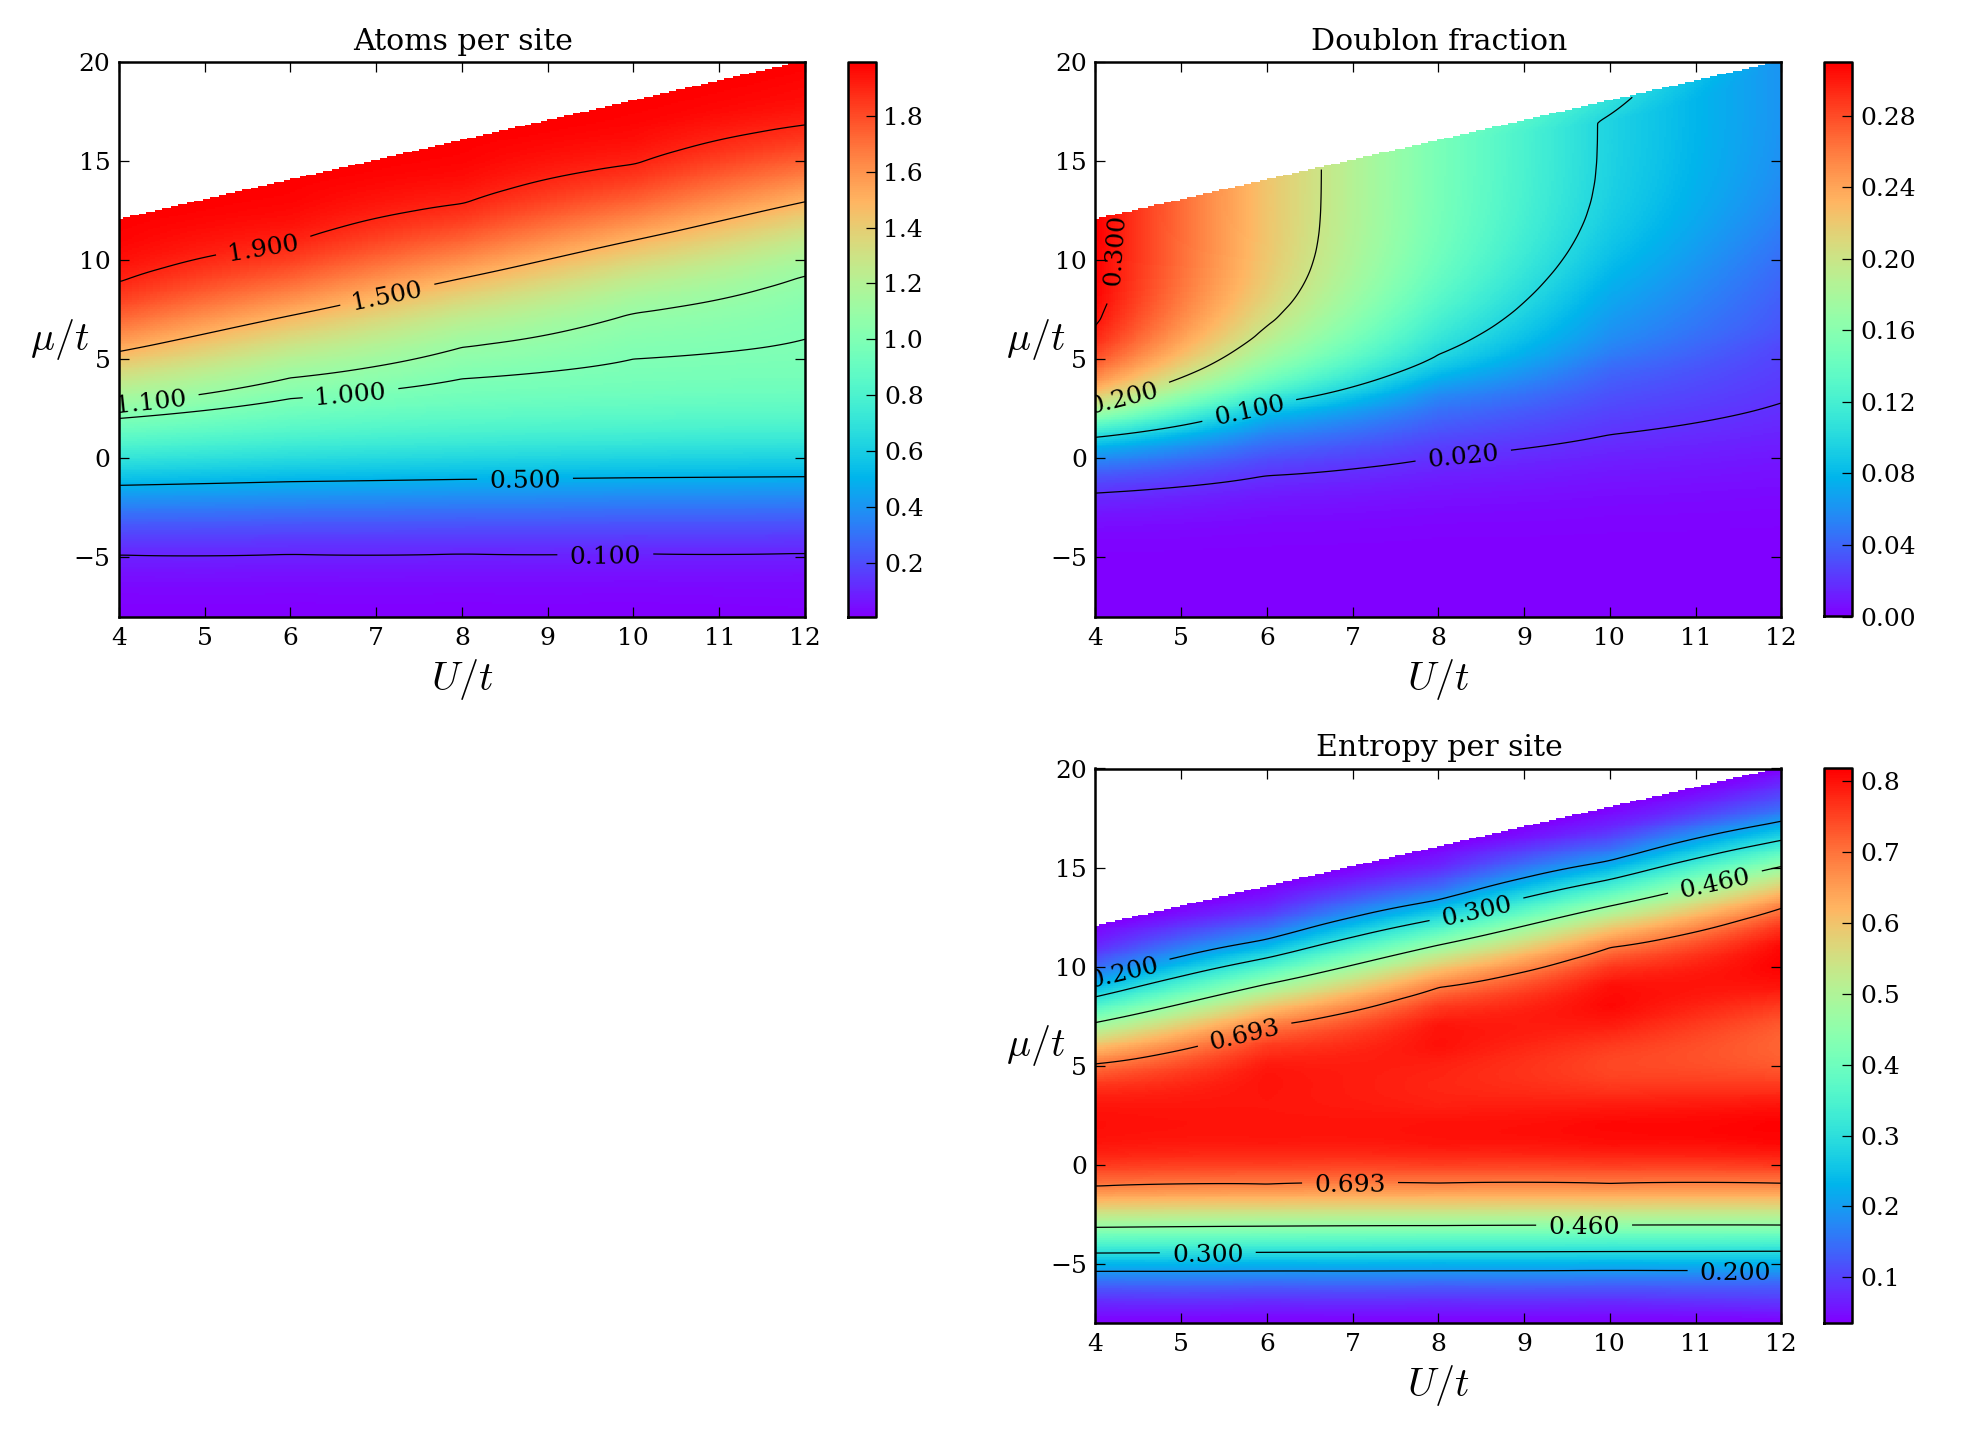
\includegraphics[width=\textwidth]{../figures/HubbardPhaseDiagram_figures/FUCHS_phasesT=10.png}
%%%%\caption[Low temperature phase diagram of the Fermi-Hubbard model]{\small
%%%%From~\cite{Fuchs2011}} \label{fig:fuchs01}
%%%%\end{figure}
%%%%   
%%%%\begin{figure}
%%%%\centering 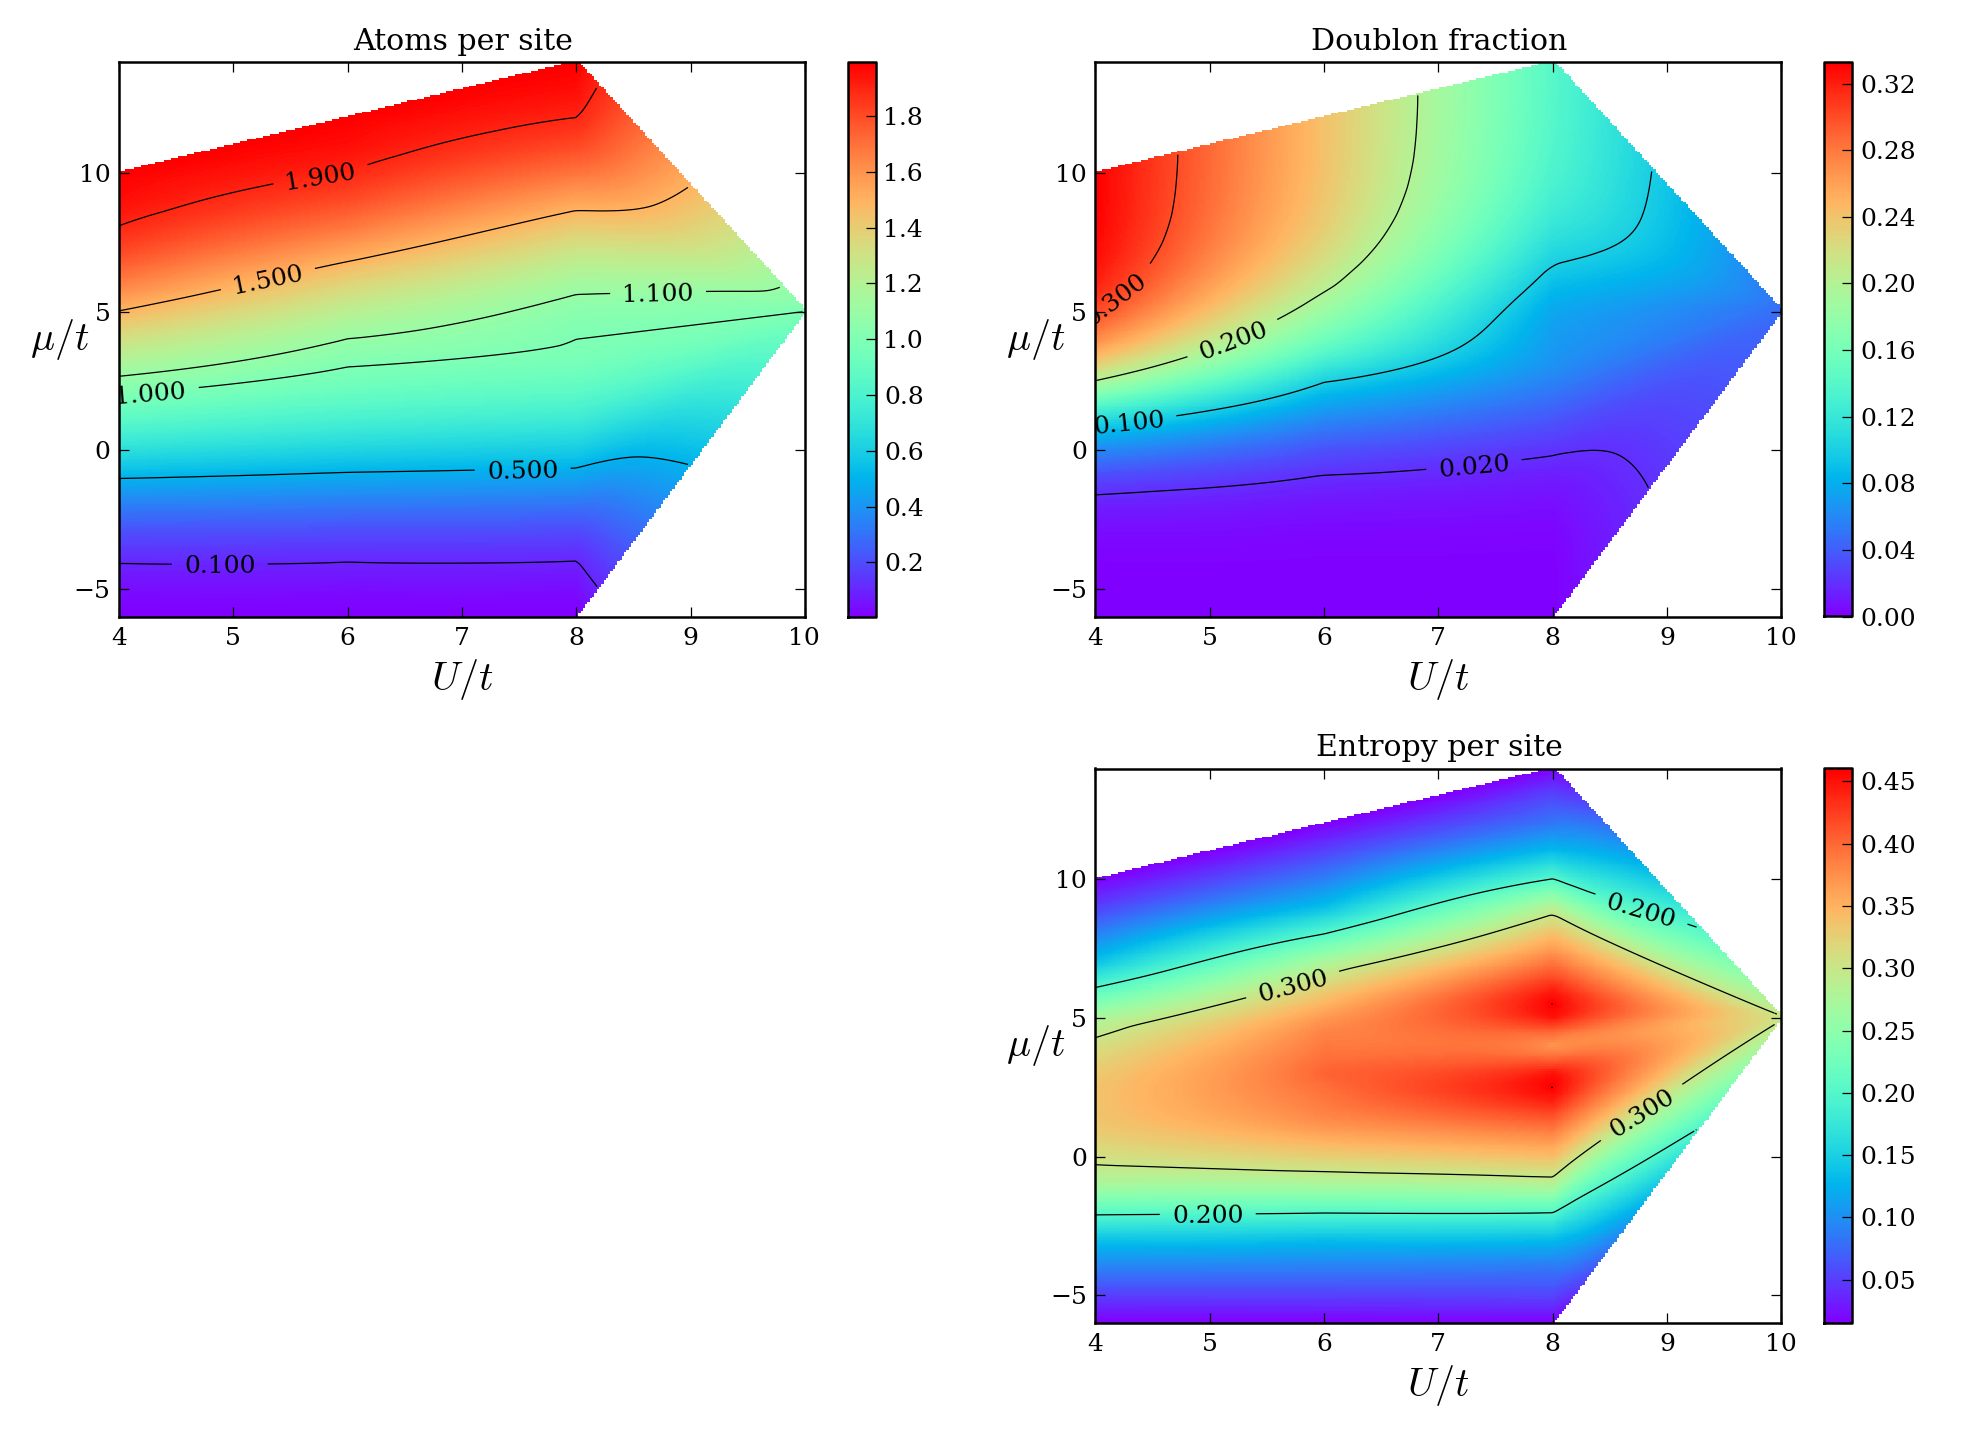
\includegraphics[width=\textwidth]{../figures/HubbardPhaseDiagram_figures/FUCHS_phasesT=3.png}
%%%%\caption[Low temperature phase diagram of the Fermi-Hubbard model]{\small
%%%%From~\cite{Fuchs2011}} \label{fig:fuchs03}
%%%%\end{figure}
%%%%
%%%%
%%%%\subsection{ Local density approximation }
%%%%
%%%%
%%%%
%%%%The phase diagrams calculated in the two previous sections assume a homogeneous
%%%%lattice.  In our experiment the lattice has an underlying confining potential,
%%%%which can be dealt with by considering a local chemical potential at each point
%%%%in the trap given by
%%%%\begin{equation}
%%%% \mu(\bv{r}) = \mu - V(\bv{r}) 
%%%%\end{equation}
%%%%An homogeneous lattice phase diagram can be used to obtain the local density,
%%%%local entropy, and local double occupancy at any point in our system by using
%%%%as inputs the local chemical potential,  the local value of the tunneling
%%%%matrix element and the local value of the on-site interaction.  
%%%%
%%%%The methods used to calculate the phase diagrams are related to the validity of
%%%%the local density approximation.   We recall that in the high temperature
%%%%series expansion, the $n^{\text{th}}$  term corresponds to a particle staring
%%%%at a certain site, tunneling $n$ times and then coming back to its original
%%%%site.  If $\sqrt{n}$ becomes comparable to the length scale of variations in
%%%%the confining potential, then the local density would not be a suitable
%%%%description of the system, because in those $n$ steps the particle can sample a
%%%%very different confining potential.  
%%%%
%%%%Similarly, in the cluster dynamical mean-field theory, results are obtained for
%%%%finite sized clusters of various sizes and then extrapolated to the infinite
%%%%size limit~\cite{Fuchs2011}.  At low temperatures, the system develops
%%%%long-range correlations, so large clusters are required to approximate the
%%%%system.   If the local site energy varies considerably over the size of a
%%%%cluster then the local density approximation will break down.   
%%%%
%%%%
%%%%
%%%%
%%%%
%%%% 
%%%%\subsubsection { High temperature series expansion, band and Mott insulating states  }
%%%%\subsubsection { small t, the t-J model and antiferromagnetic ground state}
%%%%
%%%%\subsection{Modern approaches}  
%%%%
%%%%This small section aims to explain the most recent advances in our
%%%%understanding the Fermi-Hubbard model.  This includes QMC, DMFT, etc.  The aim
%%%%of this section is not to provide an introduction to these techniques but
%%%%mainly to point out the main results and serve as a bibliographic reference.  
%%%%
%%%%

\chapter{Compensated optical lattice potential}

This chapter will consist of the detailed report that I wrote on the use of the compensated optical lattice to control the density of the sample and enable evaporative cooling of the atoms in the lattice. 

%\section{Compensated optical lattice} 
%\section{Thermodynamic quantities in the local density approximation} 


\chapter{Experimental diagnostic tools} 

This chapter aims to describe in detail the different observables that are
accessible to us, and describe in a general way the setups that we use to
measure them. 

\section{Absorption imaging} 

\section{Polarization phase-contrast imaging} 

\section{Thermometry of a Fermi gas trapped in a harmonic potential} 

\section{Double occupancy measurement in an optical lattice }

\section{Bragg Scattering of light}
 
\subsection{ Non-spin sensitive: crystal structure factor}
\subsection{ Spin sensitive:  spin-structure factor} 

\chapter{Experimental setup and procedures} 

In this chapter I will go into details about the implementations of the methods
in our particular setup.  Details about calibrations and other details very
specific to our experiment will be in this chapter. 

\section{Production of a deeply degenerate $^{6}$Li spin mixture in a dimple
potential } 

\section{Compensated optical lattice potential, calibrations}

\section{Lattice loading} 

\section{Round-trip temperature measurements}

\section{Bragg scattering setup}  

\chapter{Mott insulating state in a simple cubic lattice} 

This chapter will contain the details of the paper on the incompressibility of
the Mott insulator on which I am working at the moment.  

\chapter{Antiferromagnetic correlations in the Hubbard model}

This chapter will contain the results of the AFM paper.   

%\section{Determination of the crystal structure factor using Bragg scattering}
%\section{Insulating states in an uncompensated lattice} 
%\section{Evaporative cooling in a compensated optical lattice} 
%\section{Detection of antiferromagnetic correlations in a compensated optical lattice}

\chapter{Conclusion} 

%\section{Compensated optical lattice }
%
%\chapter{Realizing the Fermi-Hubbard model with ultracold atoms}
%
%\section{Optical lattice potential}  
%
%\section{On-site interactions} 
%
%\section{Compensated lattice: Enlarging the Neel state} 
%
%
%\chapter{Measurement and diagnostic techniques}
%
%\section{Polarization phase-contrast imaging}
%
%
%\section{Thermometry} 
% 
%\section{Bragg scattering of light}
%
% 
%\chapter{Experimental apparatus}
%
%\section{Magneto-Optical Traps}
%\section{Magic Wavelength Optical Dipole Trap}
%\section{Compensated Optical Lattice}
%\section{Bragg scattering setup} 
%
%
%\chapter{Detection of antiferromagnetic correlations}




%% finally, start of your main text

% if appendices, then
%\appendix
%\chapter{Appendix}


% if Biographical sketch then
%\begin{biosketch} I was kissed by a donkey when I was 5..... and text and more
%text and even more text, lots of text, here and there, more and more text,
%with more and more descriptions of text, blah etc blah et \end{biosketch}

\bibliographystyle{osa}
% Other options for the bibliographystyle are listed below
%\bibliographystyle{unsrt}
%\bibliographystyle{unsrtnat}
%\bibliographystyle{apsrev}
\bibliography{pmd}

\end{document}

